\documentclass[conference]{IEEEtran}
\usepackage{graphicx}
\usepackage{amsmath,amssymb,amsthm}
\usepackage{booktabs}
\usepackage{array}
\usepackage{tikz}
\usetikzlibrary{arrows.meta,positioning}
\usepackage[margin=1.9cm]{geometry}
\usepackage{hyperref}
\newtheorem{lemma}{Lemma}
\newtheorem{proposition}{Proposition}

\graphicspath{{figures/}}

\title{Symmetry-Induced Observability Limits and Sensor Placement\\in a Partly Instrumented Water Network}

\author{
\IEEEauthorblockN{Authors to be supplied}
\IEEEauthorblockA{Affiliation to be supplied}
}

\begin{document}
\maketitle

\begin{abstract}
A few sensors on a water network leave some state directions undetermined. We ask which directions, and where one more sensor should go. In a six-state benchmark where only two tank levels are measured, a mirror symmetry of the graph makes the difference between two junction heads unobservable. The same argument covers every direction that a symmetry group fixing the sensors cannot distinguish. Small symmetry-breaking perturbations of the pipe conductances can restore observability, with the weakest Gramian eigenvalues growing quadratically in the perturbation size under the stated nondegeneracy conditions; perturbations that keep the symmetry restore nothing. A placement rule that adds sensors at nodes the symmetry moves removes all symmetry-induced unobservable directions with at most $\log_2|\mathcal G|$ sensors (Propositions~\ref{prop:scaling}--\ref{prop:orbit}). No estimator we tested does better than the prior-only error ($0.0695$) in the unobservable direction: ridge regression, a Kalman filter, tuned recurrent and graph networks, and interacting multiple-model (IMM) filters all stay at it. In the directions that can be recovered, tuned networks reach about half the error of ridge regression and the Kalman filter. The IMM does better still on the synthetic benchmark, but not on an EPANET-engine simulation of the same graph, where a GRU is as good or better ($0.339$ against $0.352$). On those simulations the symmetry-based rule and a weak-direction Bayesian criterion pick the same sensor pair in $14$ or $15$ of $15$ configurations, and the best single sensor for the weak direction differs from the best for total error.
\end{abstract}

\begin{IEEEkeywords}
observability, graph symmetry, sensor placement, state estimation, Kalman filtering, partially observed networks, water distribution.
\end{IEEEkeywords}

\section{Introduction}

A few sensors cannot determine the whole state of a water distribution network. Before choosing an estimator it is worth asking which state directions the sensors determine at all, and where an additional sensor should go if some are missing. Learning cannot remove structural unobservability, although prior information can support statistical inference in unobservable directions. The answer therefore bounds what any estimator can extract from the readings alone, and the placement can be decided before any data are collected.

We study both questions on a six-state benchmark with two tanks, four hidden junctions, stochastic demand, measurement noise on the tanks and recorded disturbance events. The mirror symmetry of its graph makes the difference between two junction heads unobservable from the tank readings. Conductances that break the symmetry restore observability in principle, but only weakly. The benchmark is a network-diffusion model inspired by water distribution and is not derived from hydraulic first principles; we repeat the main experiments on an EPANET-engine simulation of the same graph. All data are simulated. This is a preliminary study whose purpose is to fix the hypotheses and the evaluation protocol for measured data (Section~\ref{sec:conclusion}).

\textbf{Contributions.}
\begin{itemize}
  \item A comparison of sensor-placement rules on seven topologies and in $15$ EPANET-engine configurations. The best extra sensor depends on the objective: the junction that best recovers the weak direction is not the one that best reduces the total error (Section~\ref{sec:sensor}, Appendices~G and~I).
  \item A placement rule that adds sensors at nodes the symmetry moves and needs at most $\log_2|\mathcal G|$ sensors to remove the symmetry-induced unobservable directions, with a guarantee that covers these directions only (Proposition~\ref{prop:orbit}).
  \item A symmetry classification of the unobservable directions of a network whose symmetry group fixes the sensors, and an order-$\varepsilon^2$ law for the weakest Gramian eigenvalues under symmetry-breaking conductance perturbations of size $\varepsilon$, certified in exact arithmetic for the benchmark graph (Propositions~\ref{prop:scaling} and~\ref{prop:sym}, Section~\ref{sec:obs}). The mathematical tools are classical and the contribution is their combination for this problem.
  \item Evidence that the limit binds every estimator we tried, on the benchmark, on two other topologies with nonlinear flow and on an EPANET-engine simulation (Section~\ref{sec:antisym}), and a supporting comparison of estimators in the recoverable directions that shows how the advantage of model-based filters depends on model fidelity (Section~\ref{sec:estimators_summary}, Appendices~B, G and J).
\end{itemize}

\textbf{Organization.} Section~\ref{sec:model} defines the benchmark, Section~\ref{sec:obs} derives the observability limit and Propositions~\ref{prop:scaling}--\ref{prop:orbit}, Section~\ref{sec:results} reports the experiments, Section~\ref{sec:discussion} discusses them and Section~\ref{sec:conclusion} gives the plan for measured data. Supporting and secondary experiments are in the appendices; Appendix~A is a guide.

\section{Related Work}
\label{sec:related}

\textbf{Lyapunov certificates.} Sum-of-squares and semidefinite certificates for Lyapunov functions are studied in the Automation and Control group at Aalborg University~\cite{leth2017farkas,misra2020satellite}. We use only a linear contraction fact about the simulator's state-transition matrix (Lemma~\ref{lem:contr}) and make no stability statement about the learned observers.

\textbf{Sensor placement and state estimation in water networks.} Sensor placement in water distribution networks is usually posed as a combinatorial optimisation for contamination or leak detection~\cite{berry2005,krause2008}, and hydraulic state estimation from pressure and flow measurements is a long-standing topic~\cite{bargiela1989,preis2011}. The BattLeDIM competition provided a common benchmark for leakage detection with SCADA data~\cite{vrachimis2022}. These works use hydraulic models and detection objectives. We ask a more basic question in a controlled model with known ground truth: which directions of the state a given sensor set can recover at all, and whether learning or model knowledge changes that.

\textbf{Observability.} Observability of nonlinear systems was formalised by Hermann and Krener~\cite{hermann1977}. A rank condition says nothing about how well a direction can be estimated, so measures such as the observability Gramian, the local unobservability index and the estimation condition number~\cite{krener2009} quantify the degree of observability; we pair the Gramian with a posterior-covariance calculation and with measured estimation errors. Graph symmetries are known to produce uncontrollable (dually, unobservable) subspaces in networked systems~\cite{rahmani2009}, and the unobservable direction here is of this kind. Small Gramian eigenvalues measure how little a direction contributes to the output and underlie balanced realisations~\cite{moore1981}; the first-order behaviour of a simple zero singular value under perturbation is classical matrix perturbation theory~\cite{stewart1990}. Section~\ref{sec:obs} applies these tools to the symmetry-induced null directions of the benchmark.

\textbf{System identification and switching models.} Subspace identification estimates a state-space model directly from input--output data~\cite{vanoverschee1996}, and prediction-error identification is treated in~\cite{ljung1999}. The interacting multiple-model filter~\cite{blom1988,barshalom2001} is the classical estimator for systems with Markov-switching dynamics. Switching linear dynamical systems can be learned with variational methods~\cite{ghahramani2000} or with Bayesian nonparametric priors that infer the number of modes~\cite{fox2011}. Our label-free identification is a much simpler hard-EM switching regression on the full state and is not a contribution to switching-model learning.

\textbf{Learned observers.} Graph convolutional networks~\cite{kipf2017} and point-set encoders~\cite{pointnet,pointnetpp} are standard for relational data. Training with a Gaussian negative log-likelihood to output predictive variances is common in deep ensembles~\cite{lakshminarayanan2017}, and calibration is assessed with empirical coverage and proper scoring rules~\cite{guo2017,gneiting2007}. The Huber loss~\cite{huber1964} is the natural robust alternative to variance weighting; Appendix~\ref{sec:prob} compares against it.

\section{Model}
\label{sec:model}

\subsection{State, graph and dynamics}

The network has twelve physical nodes: two reservoirs, two primary pumps, two tanks, two booster pumps and four demand junctions. Reservoirs and pumps enter as known inputs. The dynamic state is
\begin{equation}
x_t = \begin{bmatrix}\ell_{T1}(t)\\ \ell_{T2}(t)\\ h_{J1}(t)\\ h_{J2}(t)\\ h_{J3}(t)\\ h_{J4}(t)\end{bmatrix}\in\mathbb{R}^{6\times 1},
\label{eq:state}
\end{equation}
with tank levels $\ell_{Ti}$ in metres and junction heads $h_{Jj}$. The state graph has edges $T_1{-}J_1$, $T_2{-}J_3$ and the loop $J_1{-}J_2{-}J_3{-}J_4{-}J_1$, obtained by eliminating reservoirs and pumps. This reduction is a modelling choice: the reduced matrices are defined here and are not derived from the full hydraulic equations. The Laplacian is $L=D-A$ with adjacency $A$ and degree matrix $D$.

Let $N\in\mathbb{R}^{6\times 6}$ be the signed node--edge incidence matrix and $K=\operatorname{diag}(k_1,\dots,k_6)$, $k_e>0$, the pipe-conductance matrix. The net outflow is
\begin{equation}
\begin{aligned}
\text{flow\_net}(t)&=-L_K\,h(t), \qquad h=S^{-1}x,\\
L_K&=NKN^\top\in\mathbb{R}^{6\times 6},
\end{aligned}
\label{eq:flow}
\end{equation}
where $S=\operatorname{diag}(a_{T1},a_{T2},1,1,1,1)$ holds the tank cross-sections. Dividing by $S$ converts a tank state into a head only if that state is a volume ($x_{T_i}=a_{T_i}h_{T_i}$); in the estimation experiments the cross-sections are one, so $S=I$, $x_{T_i}=\ell_{T_i}$ is the level in metres and $h=x$ (the contraction check below also tries other areas). For an undirected graph $NN^\top=D-A$, so $K=kI$ gives $L_K=kL$. The simulator uses $K=kI$ with $k=0.35$. Heterogeneous conductance draws each $k_e$ from $\mathcal U[0.25,0.45]$ with seed $2024$.

The discrete-time update is
\begin{align}
x_{t+1} &= x_t+\Delta t\big[-L_KS^{-1}x_t \\
&\qquad+u_t-d_t\big],\label{eq:dyn}\\
u_t &= k_pE\,(x^\ast-x_t),\qquad E=\operatorname{diag}(1,1,0,0,0,0),\label{eq:pump}\\
d_{j,t} &= d_0\big(1+0.5\sin(2\pi t/48)\big)+\xi_{j,t}, \\
&\qquad j\in\{J_1,\dots,J_4\},\label{eq:demand}
\end{align}
with $\Delta t=0.5$, $k=0.35$, $k_p=0.6$, $x^\ast=5$, $d_0=0.4$, $\xi_{j,t}\sim\mathcal N(0,0.05^2)$ and demand is clipped at zero. The demand noise $\xi$ enters the state transition and therefore acts as process noise; it is the only random input of the simulator besides the events. Disturbance events occur with probability $0.08$ per step and last six steps. The event types are sensor dropout (one tank reading is masked), pump trip (a tank's pump is forced off) and demand spike (a junction's demand is multiplied by four). About one third of all steps are event-active in this schedule.

\subsection{Observation}

The observation is $o_t=(y_{T1},y_{T2},0,0,0,0)$ with mask $m_t$, where $y_{Ti}=\ell_{Ti}+v_{i,t}$ and $v_{i,t}\sim\mathcal N(0,0.03^2)$. Junction entries are never observed. A dropout masks one tank at a time, so at least one tank is always observed. The comparison is matched observable information with different missing-data encodings. The learned observers receive $o_t$ only, so a dropout appears as an exact zero; tank readings stayed above $0.8$, so the zero identifies it. The ridge model receives $m_t$ explicitly. A noise-free run agrees with the recursion $x_{t+1}=Ax_t+b_t$, where $A=I-\Delta t(L_KS^{-1}+k_pE)$, to $3\times10^{-7}$ over 40 steps. Table~\ref{tab:params} lists the parameters.

\begin{table}[t]
\centering
\caption{Simulator parameters.}
\label{tab:params}
\small
\begin{tabular}{lll}
\toprule
Symbol & Value & Description \\
\midrule
$\Delta t$ & 0.5 & time step \\
$k$ & 0.35 & pipe gain (so $K=kI$) \\
$k_p$ & 0.6 & tank pump gain \\
$x^\ast$ & 5.0 & tank set-point \\
$d_0$ & 0.4 & base junction demand \\
$\sigma_d$ & 0.05 & demand noise standard deviation \\
$\sigma_v$ & 0.03 & measurement noise standard deviation \\
$p_{\text{event}}$ & 0.08 & event probability per step \\
event length & 6 & steps per event \\
\bottomrule
\end{tabular}
\end{table}

\subsection{Contraction of the linear part}

\begin{lemma}[Contraction, unit tank areas]
\label{lem:contr}
Assume $S=I$. Then $A=I-\Delta t(kL+k_pE)$ is symmetric. Its eigenvalues with the parameters above are $0.952$, $0.677$, $0.650$, $0.549$, $0.323$ and $0.149$ and $\|A\|_2=0.952<1$. In general $\|A\|_2<1$ whenever $0<\Delta t\,\mu_{\max}<2$, where $\mu_{\max}$ is the largest eigenvalue of $kL+k_pE$.
\end{lemma}

\begin{proof}
$kL+k_pE$ is symmetric and positive definite, because the kernel of $L$ is the constant vector and $E$ removes it. The eigenvalues of $A$ are $1-\Delta t\,\mu_i$, which lie in $(-1,1)$ exactly when $0<\Delta t\,\mu_i<2$. The eigenvalues listed are computed numerically from the simulator matrices.
\end{proof}

For general tank areas $S\neq I$ the matrix $A$ is not symmetric and we make no contraction claim; numerically $\|A\|_2$ stayed below one for the areas $(2,3)$ and $(5,0.5)$ we tested. The explicit update is stable while $\Delta t\,\mu_{\max}<2$. The exact limit is $k^\ast=0.838$, where $\|A\|_2$ reaches one; the simulator's $k=0.35$ lies inside it (Fig.~\ref{fig:gain}).

\begin{figure}[t]
\centering
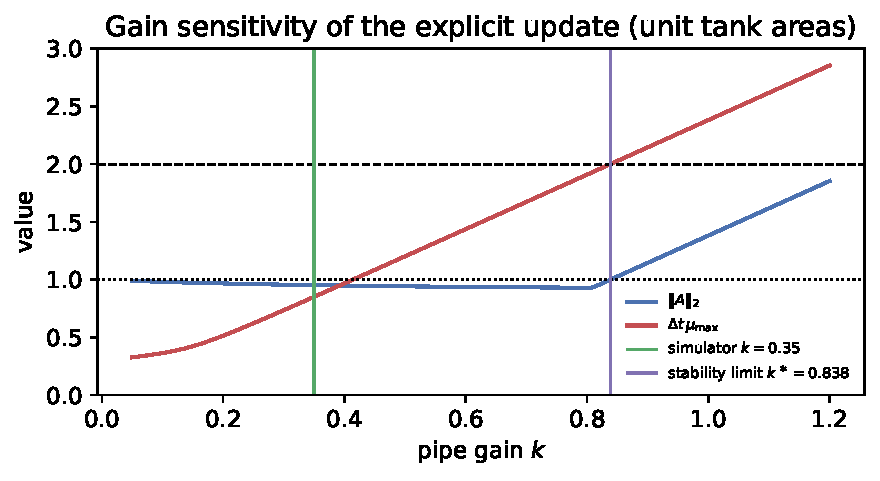
\includegraphics[width=0.55\linewidth]{fig_gain.pdf}
\caption{Gain sensitivity of the explicit update with unit tank areas.}
\label{fig:gain}
\end{figure}

\section{Observability}
\label{sec:obs}

A linear system $x_{t+1}=Ax_t$, $y_t=Cx_t$ is observable when the observability matrix $\mathcal O=[C;\,CA;\,\dots;\,CA^5]$ has rank six. Here $C$ selects the two tank states. For the homogeneous benchmark, $\mathcal O$ has rank five: its smallest singular value is zero. The null direction is $v=(0,0,0,1,0,-1)^\top$, the antisymmetric difference between $J_2$ and $J_4$. It is an eigenvector of $A$ with eigenvalue $0.650$ and $Cv=0$, so $CA^kv=0$ for all $k$. The tank sensors cannot see the difference between $J_2$ and $J_4$ under homogeneous pipes, whatever the estimator.

With heterogeneous conductance the same check gives full rank six in all $200$ random draws (each $k_e\sim\mathcal U[0.25,0.45]$). Heterogeneity therefore restores observability in principle. Full rank is not the same as useful information. The observability Gramian $W_o(T)=\sum_{k=0}^{T-1}(A^k)^\top C^\top CA^k$ quantifies how strongly each state direction appears in the observations over a horizon $T$. Its smallest eigenvalue is zero to machine precision for the homogeneous model, at both $T=6$ and $T=64$, so the condition number is infinite. For the heterogeneous draws the smallest eigenvalue is positive but small: its median is $7\times10^{-5}$ at $T=6$ and $3\times10^{-4}$ at $T=64$, with a range of $3\times10^{-9}$ to $2\times10^{-3}$. The J2-minus-J4 direction is therefore observable in principle under heterogeneity, but it contributes very little to the observations. This explains why no estimator reduces its error in practice (Section~\ref{sec:antisym}).

\textbf{Noise-normalised recoverability.} Structural observability (a rank condition), recoverability under a stated Gaussian prior (a posterior covariance) and the accuracy of an estimator under disturbances are different questions. The first two are treated analytically here and the third empirically in Section~\ref{sec:results}.

\emph{(i) Gaussian recoverability of the initial state.} For a Gaussian prior $P_0$ and measurement variance $\sigma_v^2=9\times10^{-4}$, the posterior covariance after a horizon $T$ is $P_{\text{post}}=(P_0^{-1}+W_o/\sigma_v^2)^{-1}$, computed in full without assuming that the weakest direction is an eigenvector of the prior. The randomised-start benchmark draws the initial state from independent normals with variance $0.25$, so $P_0=0.25I$ is the correct prior for that setting and is our main result.
\begin{itemize}
\item With homogeneous pipes the variance reduction along $v$ is zero and the weakest Gramian direction coincides with $v$.
\item For the $200$ heterogeneous draws the weakest direction is close to $v$ (median $|\cos|=0.998$, minimum $0.990$) and the median variance reduction along $v$ is $2.2\%$ at $T=6$ and $6.9\%$ at $T=64$, with maxima of $23\%$ and $36\%$. These are medians under the stated approximation, not bounds.
\item As a sensitivity check we used the pooled covariance of the trajectory states (variance $0.065$ along $v$), which is not a prior on the initial state (the original benchmark fixes it): the median reductions are $0.7\%$ and $2.2\%$, with maxima of $8\%$ and $14\%$.
\item Under a correlated prior, observations can reduce the variance in a dynamically unobservable direction through the correlations (a reduction of $7\times10^{-5}$ in the homogeneous case); that is statistical inference through the prior, not observability.
\end{itemize}

\emph{(ii) Empirical recoverability in the benchmark}, which includes the actual disturbances, is measured directly as the difference between an estimator's error and that of a prior-only estimator (Section~\ref{sec:antisym}); all estimators are at the prior level. The Gaussian calculation assumes noise-free dynamics and ignores the demand disturbances, which act as unmodelled noise, so it indicates how much information the sensors carry and does not predict estimator error. Heterogeneity restores observability in the algebraic sense but leaves the direction largely unrecoverable at this noise level.

\textbf{Scaling with the size of the asymmetry.} Why does algebraic observability return before useful recoverability? Write the conductances as $k_e=k(1+\varepsilon u_e)$, $u\in\mathbb R^6$, so that $A(\varepsilon)=A_0+\varepsilon A_1$ exactly, with $A_1=-\Delta t\,k\,N\operatorname{diag}(u)N^\top$ (the pump term is unchanged). Let $M_T(\varepsilon)=[C;CA;\dots;CA^{T-1}]$, so that $W_T=M_T^\top M_T$, let $v$ be the unit unobservable direction of $A_0$ ($A_0v=\lambda v$, $\lambda=0.650$, $CA_0^jv=0$), $T\ge6$ so that $M_T(0)$ has rank five, and $\Pi$ the orthogonal projector onto the complement of the range of $M_T(0)$. Define $c=\partial_\varepsilon M_T(\varepsilon)v|_{\varepsilon=0}$, the stack over $j=1,\dots,T-1$ of $c_j=\sum_{i=0}^{j-1}\lambda^{i}\,CA_0^{\,j-1-i}A_1v$.

\begin{proposition}\label{prop:scaling} (a) If $A_1v\in\operatorname{span}(v)$, then $v$ is unobservable for every $\varepsilon$ and $W_T(\varepsilon)$ is singular. (b) Let $s(\varepsilon)=\min_{y\perp v}\|M_T(\varepsilon)(v+y)\|^2$. Then $s(\varepsilon)=\varepsilon^2\|\Pi c\|^2+O(\varepsilon^3)$ and $\lambda_{\min}(W_T(\varepsilon))=s(\varepsilon)\,(1+O(\varepsilon^2))$. (c) If $\Pi c\ne0$ and $P_0=pI$, the posterior variance reduction along $v$, $1-v^\top P_{\mathrm{post}}v/p$, lies between $\kappa_1\varepsilon^2$ and $\kappa_2\varepsilon^2$ for small $\varepsilon$, with constants that depend on $p/\sigma_v^2$ and $\|\Pi c\|$. (d) For the benchmark graph, $A_1v\in\operatorname{span}(v)$ if and only if $u_3=u_6$ and $u_4=u_5$ (equal perturbations of the mirror-image pipes $J_1J_2$, $J_1J_4$ and of $J_2J_3$, $J_3J_4$), and, for $T=6$ and $T=64$ (certified in exact arithmetic), $\|\Pi c\|^2$ is a positive quadratic form in the mirror-antisymmetric part of $u$.
\end{proposition}

The proof (Appendix~\ref{app:proof}) writes $s(\varepsilon)$ as a Schur complement of the Gramian, shows that its first-order term is $\varepsilon^2\|\Pi c\|^2$ and bounds the smallest eigenvalue above and below by $s$ up to a factor $1+O(\varepsilon^2)$; the posterior variance reduction follows from the same Schur complement. Part (d) is a computation with the incidence matrix plus an exact rational certificate for the $2\times2$ form.

Part (b) is the first-order perturbation of a simple zero singular value of $M_T$~\cite{stewart1990} and part (c) is a Schur-complement identity for Gaussian posteriors. We claim no new perturbation theorem. What the proposition adds for this benchmark is the link between the two (the same Schur complement controls the smallest Gramian eigenvalue and the variance reduction, up to factors $1+O(\varepsilon^2)$ and $p/\sigma_v^2$), the identification of the perturbations that leave $v$ unobservable (the mirror-symmetric ones) and a certified nondegeneracy condition for the benchmark graph. We did not find this combination for symmetry-induced null directions in the sources we checked, but our literature search was not exhaustive.

The result is local: $\varepsilon$ small and $T$ fixed. It does not bound the remainder at the conductance spread of our heterogeneous draws ($\varepsilon\approx0.29$). It is proved for this graph and symmetry, and the nondegeneracy condition in (d) is certified in exact arithmetic for $T=6$ and $T=64$ only. Numerically, the first-order value $\varepsilon^2\|\Pi c\|^2$ matches the exact $s(\varepsilon)$ to $0.2\%$ at $\varepsilon=10^{-3}$ and $\lambda_{\min}/s-1$ is below $2\times10^{-5}$ (\texttt{proposition1\_check.py}). A sweep over $\varepsilon$ (\texttt{asymmetry\_scaling\_sweep.py}; $P_0=0.25I$, $200$ random draws of $u$ per $\varepsilon$, medians) shows that for $\varepsilon$ from $10^{-4}$ to $0.009$ the smallest eigenvalue of $W_o$ and the variance reduction along $v$ both scale as $\varepsilon^{2}$ (log--log slopes $1.97$--$2.00$ for random and reflection-breaking perturbations and $T=6$, $64$), and perturbations that keep the reflection symmetry leave both at zero to numerical precision ($<10^{-16}$). Extrapolated to the conductance spread of our heterogeneous draws, the constants give a smallest eigenvalue of order $10^{-4}$ and a variance reduction of a few per cent, in line with the values above. In practice the information about the weak direction grows only quadratically with the asymmetry, so halving the asymmetry cuts it by about four.

\textbf{Other topologies.} The unobservable direction is a consequence of graph symmetry, not of this particular graph. Table~\ref{tab:topo} gives, for seven small topologies with the same dynamics, the number of unobservable directions with homogeneous pipes and the median smallest eigenvalue of $W_o/\sigma_v^2$ at $T=64$ over $200$ heterogeneous draws. With the tanks on adjacent junctions the homogeneous system is fully observable and the weakest eigenvalue is ten times larger than for the benchmark ($2.9$ against $0.29$); symmetric attachments leave one unobservable direction (two for an eight-node ring with opposite tanks) and a weak Gramian after heterogeneity. This analysis covers observability only; the estimator comparisons were run on the original topology.

\begin{table}[t]
\centering
\caption{Observability of other topologies.}
\label{tab:topo}
\small
\setlength{\tabcolsep}{3pt}
\resizebox{\linewidth}{!}{%
\begin{tabular}{lccc}
\toprule
Topology & States & Unobs. dir. & Median $\lambda_{\min}$ \\
\midrule
Benchmark (loop, tanks on $J_1$, $J_3$) & 6 & 1 & $0.29$ \\
Tanks on adjacent junctions & 6 & 0 & $2.9$ \\
Both tanks on the same junction & 6 & 1 & $0.018$ \\
Loop with chord $J_1$--$J_3$ & 6 & 1 & $0.19$ \\
Six-junction ring, tanks opposite & 8 & 2 & $0.026$ \\
Six-junction ring, tanks adjacent & 8 & 0 & $0.19$ \\
Six-junction ring with two chords, tanks opposite & 8 & 2 & $0.0055$ \\
\bottomrule
\end{tabular}}
\end{table}

\textbf{Symmetric graphs in general.} Proposition~\ref{prop:scaling} is stated for one graph, but its mechanism is general. Let $\mathcal G$ be the group of automorphisms of the graph that fix every tank node, $\Pi_g$ the permutation matrix of $g\in\mathcal G$, $P=|\mathcal G|^{-1}\sum_{g}\Pi_g$ and $V_0=\ker P$, whose dimension is $n-m$ with $m$ the number of orbits of $\mathcal G$ on the nodes. We use the dynamics of Section~\ref{sec:model} with $S=I$ and $k_e=k(1+\varepsilon u_e)$, and write $\bar u$ for the $\mathcal G$-average of the edge perturbation $u$ (the mean of $u_{g(e)}$ over $g\in\mathcal G$).

\begin{proposition}\label{prop:sym}
(a) $V_0\subseteq N_0$, where $N_0$ is the unobservable subspace of $A_0$ (so $d=\dim N_0\ge n-m$), and $V_0$ stays unobservable for every $\mathcal G$-invariant perturbation ($u=\bar u$). (b) Let $M_T(\varepsilon)=[C;CA;\dots;CA^{T-1}]$ with $T\ge n$, let $U$ be an orthonormal basis of $N_0$ (for any graph: no symmetry is assumed here), $c=\partial_\varepsilon M_T(\varepsilon)U|_{\varepsilon=0}$, $\Pi$ the orthogonal projector onto the complement of the range of $M_T(0)$ and $H(u)=(\Pi c)^\top(\Pi c)$. Then the $d$ smallest eigenvalues of $W_T(\varepsilon)$, in increasing order, satisfy $\lambda_i(W_T(\varepsilon))=\varepsilon^2\lambda_i(H(u))+O(\varepsilon^3)$, $i=1,\dots,d$. The relative error is $O(\varepsilon)$ when $\lambda_i(H(u))>0$; when $\lambda_i(H(u))=0$ the statement is that $\lambda_i(W_T(\varepsilon))=O(\varepsilon^3)$, with no $\varepsilon^2$ term. (c) If $N_0=V_0$, then $H(u)$ depends on $u$ only through $u-\bar u$, and $H(\bar u)=0$. (d) If $H(u)\succ0$ for the perturbation at hand (it holds for generic $u$ in all the cases we checked, but is not proved in general), all $d$ weak eigenvalues are of exact order $\varepsilon^2$.
\end{proposition}

\begin{proposition}\label{prop:orbit}
Let sensors be added at a set $S$ of junctions and let $\mathcal G_S$ be the subgroup of $\mathcal G$ that fixes every node of $S$. (a) The symmetry-induced unobservable subspace of the extended system, $\ker P_S$ with $P_S$ the average over $\mathcal G_S$, has dimension $n-m(\mathcal G_S)$ and is zero if and only if $\mathcal G_S$ is trivial. (b) The orbit-breaking rule \emph{repeatedly adds a junction that the current stabiliser $\mathcal G_S$ moves} (ties broken by the weak-direction posterior criterion of Appendix~I) until $\mathcal G_S$ is trivial, and does so with at most $\lfloor\log_2|\mathcal G|\rfloor$ sensors.
\end{proposition}

Proposition~\ref{prop:sym} says that state components a symmetry cannot distinguish are unobservable; that conductance perturbations preserving the symmetry do not restore them; and that for any graph the weak eigenvalues of the unobservable directions grow like $\varepsilon^2$ under a perturbation whenever the coefficient $H(u)$ is nondegenerate, where $H(u)$ depends only on the symmetry-breaking part of the perturbation when the unobservable directions are exactly the symmetry ones. Proposition~\ref{prop:orbit} turns this into a placement rule: the sensors must break the symmetry, and the number needed is bounded as for a base of a permutation group, because each added sensor at a moved node at least halves the order of the stabiliser. This is a classical group-theoretic fact, and we do not present the rule as a new algorithm; it gives, for this class of systems, a guarantee on how few sensors remove all symmetry-induced unobservable directions. The guarantee covers only these directions. A trivial stabiliser does not make the system observable by itself, because other unobservable directions can remain, and the rule says nothing about them. Both propositions are built from classical tools (eigenvalue perturbation and Ostrowski's congruence theorem, Schur complements, the orbit--stabiliser theorem and the size bound for a base of a permutation group). The contribution is their combination for this problem: a symmetry classification of the unobservable directions, an order-$\varepsilon^2$ law for the weak Gramian eigenvalues and a placement rule with a size guarantee, checked on one family of graphs. Our literature search was not exhaustive.

Table~\ref{tab:symmetry} checks the statements on the seven topologies of Table~\ref{tab:topo} (\texttt{symmetry\_propositions\_check.py}). In every topology $n-m$ equals the observed number of unobservable directions, so $N_0=V_0$ and part (c) applies. A symmetry-preserving perturbation leaves $V_0$ unobservable (residual below $10^{-15}$). For random perturbations the $d$ smallest eigenvalues of $W_{64}$ agree with $\varepsilon^2$ times the eigenvalues of $H(u)$ to within $0.3\%$ at $\varepsilon=10^{-3}$; $H(u)$ is unchanged when the symmetric part of $u$ is removed (relative change below $10^{-8}$), and its smallest eigenvalue is positive in every draw ($\ge2.1\times10^{-7}$). The greedy rule needs at most $\log_2|\mathcal G|$ sensors, after which the homogeneous system has no unobservable direction.

The equality $N_0=V_0$ can fail. Among $400$ random connected graphs with two tank nodes and $6$--$8$ nodes, $86$ had unobservable directions: exactly the symmetry ones in $84$, and more than the symmetry ones in $2$. Part (b) does not need the equality. On these graphs its eigenvalue law holds with a relative deviation of at most $4\%$ at $\varepsilon=10^{-3}$ for the nonzero eigenvalues of $H(u)$, and in the $7$ cases with a zero eigenvalue of $H(u)$ the Gramian eigenvalue is zero to $2\times10^{-16}$.

\begin{table*}[t]
\centering
\caption{Symmetry-induced unobservable directions and orbit-breaking placement.}
\label{tab:symmetry}
\small
\resizebox{\linewidth}{!}{%
\begin{tabular}{lccccccc}
\toprule
Topology & $|\mathcal G|$ & Orbits $m$ & $n-m$ & Unobs. dir. & Greedy base & $\log_2|\mathcal G|$ & Unobs. after \\
\midrule
Benchmark (loop, tanks on $J_1$, $J_3$) & $2$ & $5$ & $1$ & $1$ & $1$ & $1.0$ & $0$ \\
Tanks on adjacent junctions & $1$ & $6$ & $0$ & $0$ & $0$ & $0.0$ & $0$ \\
Both tanks on the same junction & $2$ & $5$ & $1$ & $1$ & $1$ & $1.0$ & $0$ \\
Loop with chord $J_1$--$J_3$ & $2$ & $5$ & $1$ & $1$ & $1$ & $1.0$ & $0$ \\
Six-junction ring, tanks opposite & $2$ & $6$ & $2$ & $2$ & $1$ & $1.0$ & $0$ \\
Six-junction ring, tanks adjacent & $1$ & $8$ & $0$ & $0$ & $0$ & $0.0$ & $0$ \\
Six-junction ring with two chords, tanks opposite & $4$ & $6$ & $2$ & $2$ & $2$ & $2.0$ & $0$ \\
\bottomrule
\end{tabular}}
\end{table*}



\section{Estimation objectives}
\label{sec:belief}

\subsection{Belief, Bayesian estimate and the Kalman filter}

The belief at time $t$ is $b_t(x)=p(x_t=x\mid y_{0:t})$ and the Bayesian estimate is its mean, $\hat x_t=\mathbb{E}[x_t\mid y_{0:t}]$. The pump inputs $u_t$ are a function of the state (Eq.~\eqref{eq:pump}) and are given to no estimator; the known deterministic forcing $b_t$ (set-point and mean diurnal demand) is part of the model of the model-based filters. This mean minimizes the mean squared error over all functions of the observation history. For the linear model with Gaussian noise the belief is Gaussian and the Bayes filter is the Kalman filter~\cite{kalman1960}:
\begin{align}
\hat x_{t|t-1}&=A\hat x_{t-1|t-1}+b_{t-1},\label{eq:kf1}\\
P_{t|t-1}&=AP_{t-1|t-1}A^\top+Q,\label{eq:kf1b}\\
\nu_t&=y_t-C_t\hat x_{t|t-1},\label{eq:kf2}\\
S_t&=C_tP_{t|t-1}C_t^\top+R_t,\label{eq:kf2b}\\
G_t&=P_{t|t-1}C_t^\top S_t^{-1},\label{eq:kf3}\\
\hat x_{t|t}&=\hat x_{t|t-1}+G_t\nu_t,\label{eq:kf3b}\\
P_{t|t}&=(I-G_tC_t)P_{t|t-1}.\label{eq:kf4}
\end{align}
The innovation $\nu_t$ is the reading minus its prediction. The measurement matrix $C_t$ is time-varying: it keeps the rows of the tanks that reported at step $t$. When neither tank reports, the update is skipped and $\hat x_{t|t}=\hat x_{t|t-1}$. The RTS smoother~\cite{rts1965} adds a backward pass, $C_t^{\text{s}}=P_{t|t}A^\top P_{t+1|t}^{-1}$ and $\hat x_{t|T}=\hat x_{t|t}+C_t^{\text{s}}(\hat x_{t+1|T}-\hat x_{t+1|t})$ and uses all observations, so it is an offline reference. The only process noise of the simulator is the demand noise $\xi$ and the events add shocks that the linear Gaussian model omits, so the filters' $Q$ is an effective covariance for the demand and disturbance error, estimated from one-step residuals on seed 4242 (not an evaluation seed).

\subsection{Learned observers and the losses}

A learned observer has a hidden state $h_t=\phi_\theta(y_{0:t})$ and a readout $\hat x_t=W_{\text{out}}h_t+b_{\text{out}}$. The task loss is the mean squared error over input histories. Its ideal solution is the posterior mean, so training estimates the Bayesian estimate. The probabilistic variant adds a standard deviation output and minimizes the Gaussian negative log-likelihood
\begin{equation}
\begin{aligned}
\mathcal{L}_{\text{NLL}}=\frac{1}{BT}\sum_{b,t}\Big[&\tfrac12\Big(\frac{x_b(t)-\mu_b(t)}{\sigma_b(t)}\Big)^2\\
&+\log\sigma_b(t)\Big].
\end{aligned}
\label{eq:nll}
\end{equation}
Hidden states are handled by three tools: a recursive Bayes filter (exact for linear Gaussian models, online), a learned summary trained on the posterior-mean objective (approximate) and an RTS smoother (offline). The learned observers use the second; the classical filters use the first and third with the true model, which makes them true-transition-matrix references. The Kalman filter is exact only for linear-Gaussian models; with clipped demand and events it is an approximate estimator here.

\section{Results}
\label{sec:results}

The results follow the contributions. Section~\ref{sec:antisym} shows that no estimator recovers the unobservable direction; Section~\ref{sec:estimators_summary} summarises what the estimators do achieve in the recoverable directions and how that depends on model knowledge (details in Appendix~\ref{app:estimators}, mismatch in Appendices~B and~G); Section~\ref{sec:sensor} turns to sensor placement. The untuned architectures, the probabilistic observer, event detection and the filter-versus-smoother comparison are secondary and are in Appendices~D--F.


\subsection{Error in the unobservable direction}
\label{sec:antisym}

We measured the error in the J2-minus-J4 direction $v$ for every model (Fig.~\ref{fig:antisym}). Every neural model and the linear baseline have an error of about $0.07$ there. Dense GNN, diagonal GNN, PointNet and the probabilistic GNN are within $0.001$ of each other, and homogeneous and heterogeneous pipes do not differ significantly (dense GNN, $p=0.25$). Heterogeneous conductance makes the direction observable in principle, but none of the estimators recovers it from these sensors.

Two estimators that use no observations in this direction give the reference: the constant training mean of $e\cdot v$ and the time-dependent training mean (300 training trajectories, three test sets of 1,000). Both have error $0.0695$. The true-transition-matrix Kalman filter reaches $0.0694$ and the full-history ridge regression $0.0701$, so neither improves on the prior-only estimator within the evaluation noise. The prior-only error is thus a measured reference: under homogeneous pipes the observations are invariant under swapping $J_2$ and $J_4$, so they cannot improve the estimate of the signed difference, and every estimator is at the prior level in this error measure. Information about the magnitude of the difference or about its conditional variance is not excluded by the symmetry and was not evaluated.

\begin{figure}[t]
\centering
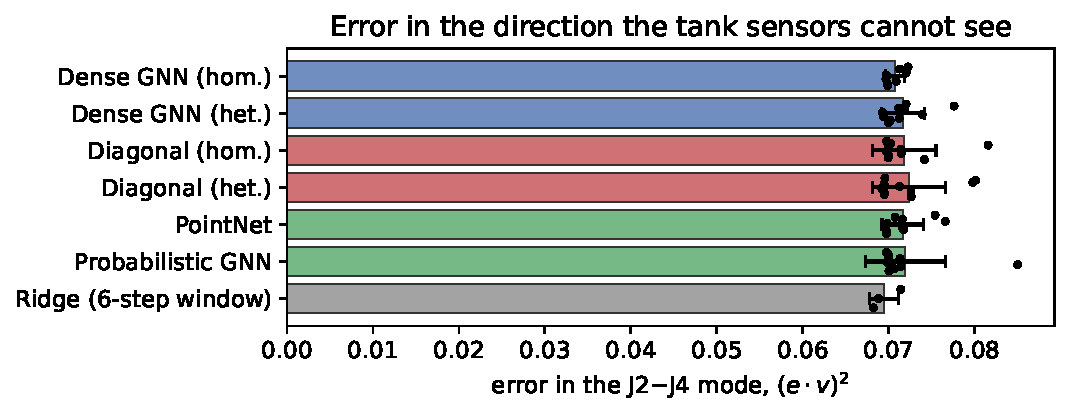
\includegraphics[width=\linewidth]{fig_antisym.pdf}
\caption{Squared error in the unit-norm J2-minus-J4 direction, $(e\cdot v)^2$ with $v=(0,0,0,1,0,-1)^\top/\sqrt2$, for each model and the six-step ridge baseline.}
\label{fig:antisym}
\end{figure}

\subsection{What the estimators achieve}
\label{sec:estimators_summary}

Two questions remain once the limit is established: does any estimator beat it, and how much do training and model knowledge matter in the directions that can be recovered? Table~\ref{tab:estimators_brief} summarises the comparison; the full comparison is in Appendix~\ref{app:estimators}. No estimator improves on the prior-only error in the weak direction (Section~\ref{sec:antisym}). In the recoverable directions, networks tuned on a validation set with the ridge inputs reach about half the error of ridge regression and of the true-transition-matrix Kalman filter, and IMM filters with the regime structure do better still on the synthetic benchmark.

The comparison is not one of equal information. The IMMs are given the regime structure and the event process (and, in the randomised-start setting, the diurnal phase); the networks and the identified IMMs use the hidden states in training; the sensor-only IMM ($0.0237$) assumes the correct structure and estimates five scalar parameters. The IMM's lead does not carry over to the EPANET-engine simulation, is lost under several shifts of the dynamics unless the estimators are rebuilt on data from the shifted system, and shrinks when the assumed event structure is wrong (Appendices~B and~G).

\begin{table}[t]
\centering
\caption{Estimators in brief: MSE on the synthetic benchmark (fixed start) and on the EPANET-engine simulation. In the J2-minus-J4 direction every estimator is at the prior-only error ($0.0695$ synthetic, about $0.050$ EPANET).}
\label{tab:estimators_brief}
\small
\begin{tabular}{lcc}
\toprule
Estimator & Synthetic & EPANET \\
\midrule
Ridge regression, 64 steps & $0.086$ & $0.489$ \\
Kalman filter, true matrix & $0.078$ & $0.470$ \\
GRU, tuned & $0.0383$ & $0.339$ \\
Graph-LSTM, tuned & $0.0374$ & --- \\
IMM, true regimes & $0.0235$ & --- \\
IMM, supervised identification & $0.0235$ & $0.352$ \\
IMM, label-free identification & $0.0236$ & $0.402$ \\
IMM, sensor-only (correct structure) & $0.0237$ & --- \\
\bottomrule
\end{tabular}
\end{table}

\subsection{Adding one junction sensor}
\label{sec:sensor}

Can one extra sensor recover the missing direction? We added one junction reading with the same noise as the tank sensors, never dropped, to the homogeneous benchmark and re-evaluated the true-transition-matrix Kalman filter (first 300 trajectories of each test set) and the full-history ridge regression (Fig.~\ref{fig:sensor}). Any junction sensor roughly halves the total error: the filter falls from $0.078$ to $0.040$--$0.041$ and the ridge regression from $0.087$ to $0.033$--$0.036$. The effect on the J2-minus-J4 direction depends on the location. A sensor at $J_1$ or $J_3$ leaves the error at the prior level (filter $0.0694$, ridge $0.0706$ and $0.0703$). This is exact for the homogeneous network: swapping $J_2$ and $J_4$ is a symmetry of the graph and of the demand model that fixes $J_1$, $J_3$ and both tanks, so readings at those nodes are invariant under the swap and cannot improve the estimate of the antisymmetric part. A sensor at $J_2$ or $J_4$ breaks the symmetry and recovers part of the direction, a $10$--$30\%$ reduction from the prior-only level (to $0.062$--$0.063$ for the filter and $0.049$--$0.050$ for the ridge regression), but much error remains under these noise and disturbance conditions. A well-placed sensor improves the estimate of the state as a whole much more than it improves this direction. The filter's own posterior variance in this direction ($0.0635$ and $0.0636$ for $J_2$ and $J_4$) agrees with its realised error; without the extra sensor the model-based variance ($0.129$) overstates the realised error ($0.069$) because the covariance is inflated by the effective process noise.

\begin{figure}[t]
\centering
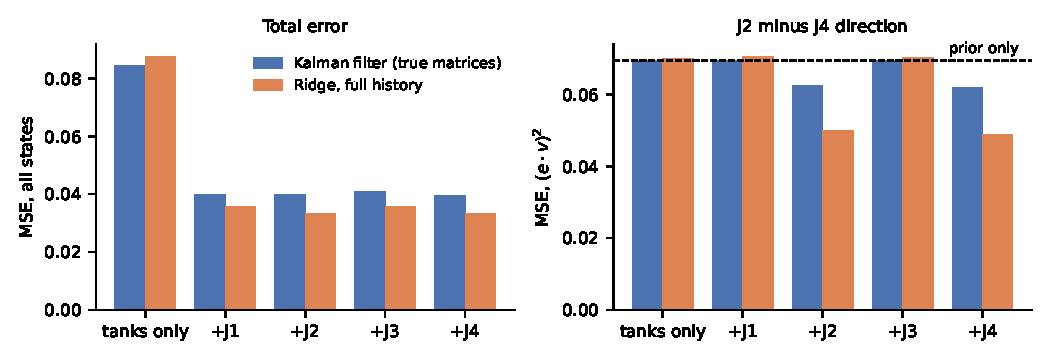
\includegraphics[width=\linewidth]{fig_sensor.pdf}
\caption{Effect of one added junction sensor on the homogeneous benchmark. Left: MSE over all states. Right: MSE in the J2-minus-J4 direction, with the prior-only level dashed. true-transition-matrix Kalman filter (300 trajectories per test set) and full-history ridge regression.}
\label{fig:sensor}
\end{figure}

\textbf{Placement rules.} Appendix~I compares five placement rules (random, symmetry, Gramian eigenvalue, Gramian trace and posterior trace) on seven topologies and $200$ heterogeneous conductance draws, with the Kalman-filter error as the score. For the weak-direction score it adds a sixth rule, the posterior variance of the initial state in the weak subspace. The symmetry rule fills the sensor budget from the nodes the symmetry moves; Proposition~\ref{prop:orbit} needs only one sensor on the benchmark graph. All are within $13\%$ of the best set on average, so for the total error the location matters by at most about $20\%$ and the noise-aware initial-state criterion does not beat a simple Gramian-trace rule. For the weak direction the choice matters much more with two sensors (random choice has $1.59$ times the best variance) and only the rule that targets the weak subspace stays within $1.06$ times the best set in every topology (Tables~\ref{tab:placement} and~\ref{tab:placement_weak}). The EPANET-engine check of these rules (Appendix~G) and the trade-off between objectives are discussed in Section~\ref{sec:discussion}.

\section{Discussion}
\label{sec:discussion}

The two tank sensors cannot see the difference between $J_2$ and $J_4$ under homogeneous pipes, and no estimator we tested recovers it. The error in that direction stays at the prior-only level ($0.0695$) for ridge regression, Kalman filters, tuned networks and IMM filters, on the benchmark, on two other topologies with nonlinear flow and on an EPANET-engine simulation. Conductances that break the symmetry make the direction observable in principle, but under the nondegeneracy conditions of Propositions~\ref{prop:scaling} and~\ref{prop:sym} the information about it grows only with the square of the asymmetry, and conductances that keep the symmetry restore nothing, so the error does not improve in practice. These statements concern these sensors, disturbances and priors; structural observability, recoverability under a prior and estimator accuracy are separate questions (Section~\ref{sec:obs}). One added sensor at $J_2$ or $J_4$ lowers the error only to $0.049$--$0.062$, and a sensor at $J_1$ or $J_3$ leaves it unchanged (Section~\ref{sec:sensor}). The BattLeDIM L-Town analysis in Appendix~C is an exploratory check on simulated data and does not validate these findings.

Where an extra sensor should go depends on what is being estimated. With one added sensor, a junction that breaks the symmetry ($J_2$ or $J_4$) is best for the weak direction in all $15$ hydraulic configurations, whereas a central junction ($J_1$ or $J_3$) is best for the total error in all $15$ (in every run); targeting the weak direction raises the total-error ratio from $1.29$ (random choice) to $1.45$. With two added sensors the pair $\{J_2,J_4\}$ is best for both objectives on this graph. The symmetry rule, which places the sensors at nodes the symmetry moves, picks that pair in all $15$ configurations of every run, and so does the weak-direction Bayesian criterion with the nominal model; with the fitted model it does so in $14$ or $15$ of the $15$ (Table~\ref{tab:hydraulic_repeats}). On this graph the stopping rule of Proposition~\ref{prop:orbit} is already met after one sensor ($|\mathcal G|=2$ and either $J_2$ or $J_4$ makes the stabiliser trivial), so the two-sensor experiments use the symmetry rule with the full budget, a choice the proposition does not cover. The hydraulic experiment therefore supports symmetry-informed placement but shows no advantage of the Bayesian criterion over it. The Bayesian criterion matters where no exact symmetry exists: in the linear-Gaussian study (Table~\ref{tab:placement_weak}) its worst case over topologies is $1.06$ times the best set, against $1.57$ for the symmetry rule, and generic criteria (Gramian eigenvalue, posterior trace over all states) fail in both settings when computed from a model that does not break the symmetry. Sensors at both $J_2$ and $J_4$ measure the two quantities whose difference is the target, so the near-noise-level error of that pair is expected. The experiment shows that the criteria find this pair, not that an estimator reconstructs an inaccessible state from indirect readings. It also uses one graph, a ridge regression trained on simulated hidden heads, and heterogeneity through pipe diameters only (Tables~\ref{tab:placement}, \ref{tab:placement_weak} and~\ref{tab:placement_hyd}).

Tuned networks reach about half the error of ridge regression and of the Kalman filter, which uses a single noise covariance for what is a mixture of regimes. IMM filters that use the regime structure do better still on the synthetic benchmark ($0.022$--$0.027$), including when their dynamics are identified without regime labels or from the tank readings alone. These comparisons do not give the estimators the same information. The IMMs have the regime structure, the networks and the identified IMMs use hidden states in training, and the sensor-only identification assumes the correct structure with five free parameters (Appendix~B); it does not need starting values near the truth: from broad absolute ranges the start with the highest training likelihood reaches $0.0234$--$0.0237$ in all three seeds, although only some starts converge. The IMM's lead does not carry over to the EPANET-engine simulation, where the GRU ($0.339$) is below the supervised IMM ($0.352$), the label-free IMM ($0.402$), the Kalman filter ($0.470$) and ridge regression ($0.489$). It also disappears under several shifts of the dynamics and returns only if the estimators are rebuilt on data from the shifted system (Table~\ref{tab:adapt}). The IMM then needs few trajectories because only five parameters of a correctly structured model are refitted, which says nothing about sample efficiency in general. A single-regime Kalman filter fitted by likelihood fails because the likelihood prefers an inflated noise level that no single regime can represent (Appendix~B). All comparisons are exploratory and tied to these simulators and training protocols.

Appendices~D and~E report the comparison of untuned architectures, the probabilistic GNN (whose advantage over a plain GNN is largely explained by per-sample weighting of the loss, and whose intervals fall below nominal coverage during pump trips and demand spikes because its predicted uncertainty hardly changes between regimes) and event detection.

\section{Limitations}

All results come from simulation. The benchmark is a linear network-diffusion model, not derived from hydraulic first principles, with six states and one topology in the main experiments. The estimator comparison was repeated on two other topologies and with a simple nonlinear flow law (five seeds, hyper-parameters re-selected on a small grid) and on an EPANET-engine simulation of the same graph (Appendix~G). That simulation reproduces the unobservable direction and the networks' advantage over ridge regression, but not the IMM's advantage over networks. The $J_2$-minus-$J_4$ direction follows from the symmetry of the graph (Section~\ref{sec:obs}). Field data are needed for claims about real networks.

The estimators do not all have the same information. The networks use the hidden junction states as training targets. The IMM has the true event process and, in the randomised-start setting, the phase. Supervised identification uses regime labels and hidden states; label-free identification uses hidden states and a BIC-selected number of regimes, is sensitive to that number (Appendix~B) and was run only with a fixed start. A deployed observer would have none of these. Sensor-only identification assumes the graph, the regime structure, the event probabilities, the spike multiplier, the set-point and the diurnal profile, and estimates five scalar parameters of a model class that contains the data-generating process; its error grows when the assumed structure is wrong. A generic switching model identified from the tank readings alone, for example by subspace identification, was not run, so the networks' advantage over the single-regime Kalman filter is partly an advantage over a model with one noise regime.

The simulated events are mutually exclusive, last exactly six steps and come from seven predefined regimes, which probably makes regime identification easier than in a real system. Event duration, rate and overlap were varied only as test-time shifts of estimators built on the nominal benchmark, without retraining or re-identification (Appendix~B), and no regime changes were added. Adaptation was tested only for three shifts of the dynamics parameters (pump gain $\times0.8$, flow gain $\times0.8$ and $\times1.2$; Table~\ref{tab:adapt}).

No hypotheses were specified in advance and the comparisons are not adjusted for multiplicity, so all of them are exploratory. We do not claim statistical equivalence between estimators or a general ranking; the rankings depend on this simulator. The ridge baselines are single fits. The tuned networks come from small grids ($14$ temporal and $4$ graph configurations, one seed each), one training length and five training seeds, and the architectures are only partly parameter-matched. The main comparison uses $900$ test trajectories ($300$ in the IMM sensitivity analysis and $150$ in the label-free validation). Each robustness shift has one test set and three GRU seeds, the multi-start identification uses three seeds per structure, and the calibration-by-event analysis uses five of ten seeds and treats per-state errors as independent in the weak direction.

The hydraulic estimator comparison (Appendix~G) is a single configuration with homogeneous pipes and three GRU seeds. The hydraulic placement study uses $15$ configurations (three homogeneous, $12$ with heterogeneous pipe diameters) and one estimator. Its numbers depend on the computing environment. Five reruns on Linux gave identical output, which Table~\ref{tab:placement_hyd} reports. A first run and two reruns on Windows differed from it, and from each other, for the rules that depend on the fitted model (Appendix~G, Table~\ref{tab:hydraulic_repeats}): the posterior-trace rule with the fitted model had a ratio of $1.83$ on Linux against $1.75$, $3.29$ and $3.30$ on Windows, and the weak-direction posterior rule chose $\{J_2,J_4\}$ in $14$ or $15$ of the $15$ configurations. We have not isolated the cause. The realised best sets, and so the trade-off between the two objectives, were identical in all runs. The Kalman-filter placement study uses one extra sensor with the tank noise level, homogeneous pipes and the first $300$ trajectories of each test set. The original spatial-encoder and calibration results refer to untuned networks. Earlier stability pass rates from drafts of this work are invalid and are not reported.

\section{Conclusion}
\label{sec:conclusion}

A graph symmetry that fixes the sensors makes the state components it cannot distinguish unobservable, and no estimator we tested beats the prior-only error in those directions. Symmetry-breaking conductances restore observability only weakly: under the nondegeneracy conditions of Propositions~\ref{prop:scaling} and~\ref{prop:sym} the information grows with the square of the asymmetry, and conductances that keep the symmetry restore nothing.

Where an extra sensor should go depends on the objective. With two sensors the pair $\{J_2,J_4\}$ is best for both the weak direction and the total error; with one, the best junction for the weak direction ($J_2$ or $J_4$) is not the best for total accuracy ($J_1$ or $J_3$). A symmetry rule that places the sensors at nodes the symmetry moves chose the same pair as a weak-direction Bayesian criterion in $14$ or $15$ of the $15$ hydraulic configurations, depending on the run. Proposition~\ref{prop:orbit} bounds the number of sensors needed to break the symmetry (one on this graph) but not the choice of a second sensor, so the experiments support symmetry-informed placement and show no advantage of the Bayesian criterion over it.

In the directions that can be recovered, tuned networks reach about half the error of ridge regression and of the Kalman filter. IMMs do better still on the synthetic benchmark when the regime structure and parameters are right, but not on the hydraulic simulation (GRU $0.339$, supervised IMM $0.352$), not under several shifts of the dynamics unless the estimators are rebuilt on data from the shifted system, and not when the assumed event structure is wrong.

These results come from a preliminary simulation study and say nothing yet about field performance. Real data will not provide the hidden junction heads, so the MSE metrics, the networks' state targets and the full-state identification of the IMMs used here cannot be reused as they stand. The protocol for the measured-data study is therefore:
\begin{itemize}
\item evaluate every estimator on \emph{held-out measured sensors} (pressure or level readings withheld from the estimator), with the same prior-only reference as here;
\item train only on observed channels, and identify the IMM from the tank readings alone, with the regime structure assumed and then perturbed as in Appendix~B;
\item keep every estimator at its nominal (design) parameters and, separately, rebuilt on data from the same system, to separate the value of model knowledge from the value of adaptation;
\item choose the sensor sets by the rules of Appendix~I and compare predicted with measured held-out error.
\end{itemize}

The hypotheses to be tested were fixed in advance; each is listed with the outcome that would count against it.
\begin{enumerate}
\item \emph{Recoverability limit.} With sensors placed symmetrically, no estimator improves on the prior-only error in the directions the symmetry analysis marks as unobservable. It would be contradicted by an estimator that clearly beats the prior-only error on a held-out sensor in such a direction without any sensor that breaks the symmetry.
\item \emph{Ranking depends on model fidelity.} Tuned learned estimators beat a single-regime Kalman filter on the same inputs, and a regime-aware model-based estimator matches or beats them only after its parameters are identified from the same system. It would be contradicted by a regime-aware estimator at nominal parameters that beats the learned estimators.
\item \emph{Placement depends on the objective.} With one extra sensor the junction that most reduces the error in the weak direction differs from the junction that most reduces the total error, and with two extra sensors the pair that breaks the symmetry is best for both. It would be contradicted by one junction being best for both objectives with a single sensor.
\item \emph{Model-guided placement.} The linearised recoverability model ranks candidate sensor sets in the same order as the measured held-out error (rank correlation clearly above zero, as in Appendix~C), and orbit-breaking sets are not worse than the best set found by search. It would be contradicted by a rank correlation near zero.
\end{enumerate}
Further work includes a detector for sensor dropouts and intervals that widen during disturbances, which the probabilistic GNN of Appendix~E does not provide.

\section*{Code and Data Availability}
Code and raw outputs are in \texttt{code/} and \texttt{results/}; the script names state what each computes. The repository is at \url{https://github.com/m-fol/water-system}.

\appendices

\section{Tuning grids}

\begin{table}[t]
\centering
\caption{Guide to the appendices.}
\label{tab:appendix_guide}
\small
\setlength{\tabcolsep}{4pt}
\begin{tabular}{@{}c>{\raggedright\arraybackslash}p{3.7cm}>{\raggedright\arraybackslash}p{2.8cm}@{}}
\toprule
App. & Content & Supports \\
\midrule
A & Tuning grids & tuned networks (Appendix~\ref{sec:tuned}) \\
B & IMM specification; label-free and sensor-only identification; robustness and adaptation & IMM results, mismatch limits \\
C & BattLeDIM L-Town (simulated data) & placement ranking \\
D & Untuned architectures, GNN controls & original comparison \\
E & Probabilistic GNN: calibration, event detection & uncertainty results \\
F & Filter against smoother & Kalman baselines \\
G & EPANET-engine simulation: estimators and sensor placement & hydraulic check \\
H & Proofs of Propositions~\ref{prop:scaling}--\ref{prop:orbit} & Section~\ref{sec:obs} \\
I & Sensor-placement rules, linear-Gaussian study & Section~\ref{sec:sensor} \\
J & Estimator comparison in detail & Section~\ref{sec:estimators_summary} \\
\bottomrule
\end{tabular}
\end{table}
Hyper-parameter grids and validation MSE (500 validation trajectories, seed 123, one training seed per configuration; selected configurations in bold). The temporal networks and the graph estimator were trained for 4,000 Adam steps of batch 32 on 8,000 fixed trajectories with cosine learning-rate decay and gradient clipping and the best validation checkpoint (every 250 steps) was kept. Hidden size is the recurrent or hidden width; for the graph estimator the first number is the graph-convolution width.

\begin{table}[t]
\centering
\caption{Tuning grids and validation MSE (fixed start).}
\label{tab:grid}
\small
\setlength{\tabcolsep}{3pt}
\resizebox{\linewidth}{!}{%
\begin{tabular}{lcccc}
\toprule
Model & Hidden & Learning rate & Parameters & Validation MSE \\
\midrule
GRU & 128 & 0.001 & 52230 & $0.0438$ \\
GRU & 64 & 0.003 & 13830 & $\textbf{0.0361}$ \\
Linear recurrent & 64 & 0.003 & 4806 & $0.0665$ \\
Linear recurrent & 64 & 0.01 & 4806 & $\textbf{0.0664}$ \\
Linear recurrent & 16 & 0.003 & 438 & $0.0670$ \\
Linear recurrent & 16 & 0.01 & 438 & $0.0665$ \\
LSTM & 128 & 0.001 & 69382 & $0.0600$ \\
LSTM & 128 & 0.003 & 69382 & $\textbf{0.0360}$ \\
LSTM & 32 & 0.001 & 5062 & $0.0711$ \\
LSTM & 32 & 0.003 & 5062 & $0.0469$ \\
MLP (16 steps) & 256 & 0.001 & 83974 & $0.0419$ \\
MLP (16 steps) & 256 & 0.003 & 83974 & $\textbf{0.0388}$ \\
MLP (16 steps) & 64 & 0.001 & 8710 & $0.0533$ \\
MLP (16 steps) & 64 & 0.003 & 8710 & $0.0479$ \\
Graph-LSTM (gc 16, LSTM 64) & 64 & 0.003 & 29174 & $0.0483$ \\
Graph-LSTM (gc 32, LSTM 64) & 64 & 0.003 & 33862 & $\textbf{0.0369}$ \\
Graph-LSTM (gc 32, LSTM 128) & 128 & 0.003 & 92102 & $0.0377$ \\
Graph-LSTM (gc 32, LSTM 128) & 128 & 0.001 & 92102 & $0.0686$ \\
\bottomrule
\end{tabular}}
\end{table}

On the other settings (ring with opposite tanks, ring with adjacent tanks, nonlinear flow) the GRU and graph-LSTM were re-selected from a grid of three GRU configurations (hidden 64 at $3\times10^{-3}$, 128 at $10^{-3}$, 128 at $3\times10^{-3}$) and four graph-LSTM configurations (graph-convolution width and LSTM width $(16,64)$, $(32,64)$, $(32,128)$ at $3\times10^{-3}$ and $(32,64)$ at $10^{-3}$), one seed each, on the validation set of each setting; the same configuration won in all three settings (GRU: 128 hidden, learning rate $3\times10^{-3}$; graph-LSTM: $(32,128)$, $3\times10^{-3}$). Validation scores are in \texttt{results/topology\_neural.json}.

\section{IMM specification and sensitivity}
\label{sec:imm}

\textbf{Events in the simulator.} At most one event is active at a time. A new event can start only when none is active, with probability $0.08$ per step; its type (dropout, pump trip or demand spike) is uniform and its node is uniform among the two tanks (dropout, pump trip) or the four junctions (demand spike). Every event lasts exactly six steps and a new event can start on the step an event ends. Events therefore never overlap (none among the 7,487 simulated events in \texttt{kalman\_imm\_checks.py}) and a dropout blocks the onset of other events while it lasts.

\textbf{Regimes and transition probabilities.} The IMM has seven regimes: calm, a pump trip at either tank, a demand spike at either junction. A pump trip removes the pump term of that tank, a demand spike multiplies the demand and its noise at that junction by four and dropouts do not change the dynamics, so they are known from the masks and merged with calm. Because events never overlap, one active regime at a time is exact. From calm the onset probabilities are $0.08/6$ for each pump trip and $0.08/12$ for each demand spike (the event probability times the uniform type and node probabilities) and an event ends with probability $1/6$ per step, a geometric approximation of the fixed six-step duration; the approximation ignores that dropouts block onsets. \textbf{Causality.} The filter uses only observations up to the estimation time: altering the observations after step $t_0$ did not change the estimates up to $t_0$ in any of 60 perturbation checks.

\textbf{Sensitivity.} Table~\ref{tab:imm_sens} varies the transition assumptions and replaces the geometric approximation by an exact-duration model that tracks the age of the event (49 models: regime by age, with dropouts as two further event types).

\begin{table}[t]
\centering
\caption{IMM sensitivity (fixed start, known start, 300 trajectories).}
\label{tab:imm_sens}
\small
\begin{tabular}{lc}
\toprule
Variant & MSE \\
\midrule
Base (onsets as simulated, exit probability $1/6$) & $0.0242$ \\
Onset probabilities $\times0.5$ & $0.0242$ \\
Onset probabilities $\times2$ & $0.0249$ \\
Exit probability $1/3$ & $0.0240$ \\
Exit probability $1/12$ & $0.0250$ \\
Exact event duration (age-tracking, 49 models) & $\mathbf{0.0207}$ \\
Identified from training data (labelled regimes) & $0.0246$ \\
\bottomrule
\end{tabular}
\end{table}

The IMM is insensitive to the transition assumptions (changes within $3\%$) and modelling the exact duration lowers its error by $14\%$, so the geometric approximation costs some accuracy but does not drive the comparison with the networks.

\subsection*{Label-free full-state identification: validation}
The switching model is identified without regime labels from 2,000 training trajectories with the full hidden state: a single affine model $x_t=Ax_{t-1}+c_0+c_1\sin(2\pi t/48)+c_2\cos(2\pi t/48)$ is fitted, its one-step residuals are clustered into $K$ groups with k-means++ (best of three restarts by training log-likelihood) and hard EM (25 iterations) refits each group's model and covariance and reassigns each transition to the group with the highest Gaussian log-likelihood. The regime transition matrix comes from the inferred label sequences and the measurement variance from the training residuals; the IMM then uses only the tank readings and masks (fixed start, known start). Because identification uses all six hidden states, we call it label-free \emph{full-state} identification: it is not sensor-only.

\textbf{Validation protocol.} For each $K\in\{3,5,7,8,9,10,11,12\}$ the identification was repeated with five independent seeds (training trajectories and k-means initialisations). The true regime labels play no role in identification. To evaluate the inferred groups, each group is matched to the true regime that holds most of its \emph{training} transitions (majority vote) and \emph{held-out} transitions (100 test trajectories, seed 777) are assigned to groups by maximum likelihood; purity is the share of held-out transitions in groups with at least 100 training transitions whose true regime equals the group's matched regime (these groups contain all held-out transitions) and the adjusted Rand index compares the held-out assignment with the true labels. The IMM error is measured on 150 test trajectories (50 from each test seed). Table~\ref{tab:labelfree} lists, for each $K$ and over the five seeds: the number of groups with at least 100 training transitions (Groups); the held-out purity, as mean (minimum over seeds); the smallest number of the seven true regimes represented in any seed (Regimes); the held-out adjusted Rand index (ARI); the IMM MSE as mean [min, max]; and the mean MSE in the unobservable $J_2$--$J_4$ direction. On the same 150 trajectories the true-regime IMM has MSE $0.0264$ ($J_2$--$J_4$: $0.0804$) and supervised identification $0.0266$.

\begin{table}[h]
\centering
\caption{Label-free full-state identification by number of groups $K$.}
\label{tab:labelfree}
\small
\setlength{\tabcolsep}{3pt}
\resizebox{\linewidth}{!}{%
\begin{tabular}{cccccc c}
\toprule
$K$ & Groups & Held-out purity & Regimes & ARI & IMM MSE & $J_2$--$J_4$ \\
\midrule
3 & 3--3 & $0.8700$ ($0.8408$) & 3 & $0.751$ & $0.2706$ [$0.0426$, $1.1325$] & $1.3881$ \\
5 & 5--5 & $0.9434$ ($0.9423$) & 5 & $0.989$ & $0.0348$ [$0.0283$, $0.0413$] & $0.1117$ \\
7 & 6--7 & $0.9704$ ($0.9409$) & 5 & $0.995$ & $0.0330$ [$0.0271$, $0.0410$] & $0.1009$ \\
8 & 6--7 & $0.9831$ ($0.9703$) & 6 & $0.997$ & $0.0333$ [$0.0265$, $0.0411$] & $0.1058$ \\
9 & 6--7 & $0.9938$ ($0.9703$) & 6 & $0.998$ & $0.0286$ [$0.0264$, $0.0370$] & $0.0922$ \\
10 & 7--7 & $0.9997$ ($0.9997$) & 7 & $0.999$ & $0.0265$ [$0.0264$, $0.0267$] & $0.0807$ \\
11 & 7--7 & $0.9997$ ($0.9997$) & 7 & $0.999$ & $0.0265$ [$0.0264$, $0.0267$] & $0.0806$ \\
12 & 7--7 & $0.9997$ ($0.9997$) & 7 & $0.999$ & $0.0265$ [$0.0264$, $0.0266$] & $0.0806$ \\
\bottomrule
\end{tabular}}
\end{table}

\textbf{Selection of $K$.}
\begin{itemize}
\item \emph{Criterion.} The number of groups was chosen by BIC computed from the training log-likelihood ($-2\log L+75K\ln N$, with 75 free parameters per regime: the $6\times9$ affine coefficients ($36$ for $A$ and $18$ for the constant and the two diurnal terms) and the $21$ distinct entries of the $6\times6$ covariance; $N=2000\times64=128{,}000$ training transitions), among the eight candidates above. The selected values are seed 0: $K=9$, seed 1: $K=9$, seed 2: $K=8$, seed 3: $K=8$, seed 4: $K=9$. Here $\log L$ is the hard-assignment (classification) log-likelihood at the last EM iteration, which flatters the fit relative to a marginal mixture likelihood, so BIC is a heuristic. The regime transition probabilities ($K(K-1)$ free parameters) and the group frequencies ($K-1$) are not in the penalty; adding them does not change the selected $K$ in any seed.
\item \emph{Error.} With the selected $K$ the IMM reaches $0.0265$ on the 150 test trajectories in every seed (range $0.0264$--$0.0267$), which differs from the true-regime IMM ($0.0264$) and from supervised identification ($0.0266$) on the same trajectories by at most $0.0002$.
\item \emph{Regime recovery.} Each of the five selected models recovers all seven regimes (held-out purity $99.97\%$), but this reflects BIC discarding poorer fits: at $K=8$ only two of five seeds and at $K=9$ four of five recover all seven regimes, so recovery of every regime should not be assumed. BIC picks $K=8$ or $9$, not $10$--$12$, which give the same error because the extra groups are empty. For $K\ge10$ all seven regimes are recovered in every seed (held-out purity $99.97\%$); for $K=9$ one of five seeds recovers only six regimes (held-out purity $99.4\%$ on average, minimum $97.0\%$); for $K\le7$ regimes are merged, the IMM error rises ($0.0348$ at $K=5$, $0.0330$ at $K=7$) and $K=3$ is unstable (up to $1.13$). The training and held-out purities agree to within $0.1$ points for $K\ge8$, so the group structure is not an artefact of fitting the training trajectories.
\item \emph{Unobservable direction.} The poorly identified models ($K\le9$) are worse than the true-regime IMM on the same trajectories ($0.0922$ and above, and $1.39$ at $K=3$, against $0.0804$); for $K\ge10$ the error equals the true-regime value ($0.0807$).
\end{itemize}

The result is strong because identification uses the hidden states: events are visible in the residuals of the true state, so separating the regimes is easy. Label-free identification of the model structure from the tank readings alone, which is the setting of a deployed observer, is a harder problem that we did not test; the sensor-only experiment below identifies only scalar parameters of an assumed structure.

\subsection*{Sensor-only identification of the model parameters}
We identified the IMM from the tank readings and masks alone, with no hidden junction states and no regime labels. The experiment is grey-box: the graph, the seven-regime structure, the event onset and exit probabilities, the spike multiplier ($4$), the tank set-point, the diurnal profile and the fixed start are assumed known, and five scalar parameters are estimated, namely the flow gain $k$, the pump gain, the base demand, the demand-noise standard deviation $\sigma_d$ and the measurement-noise standard deviation $\sigma_v$. The estimates maximise the IMM marginal likelihood of the readings of 60 training trajectories (Nelder--Mead on the logarithms of the parameters, at most 220 iterations), starting from the true values multiplied by independent random factors in $[0.6,1.5]$, for five independent seeds (training trajectories and starting points). The IMM with the identified parameters reaches an MSE of $0.0237$ (range $0.0234$--$0.0242$) on the 900 common test trajectories, against $0.0235$ at the true parameters; in the unobservable direction it stays at the prior-only level ($0.0694$). Table~\ref{tab:sensor_only} gives the relative errors of the estimates in percent. $k$, the pump gain, the base demand and $\sigma_v$ are recovered to within $1.3\%$, while $\sigma_d$ is only weakly identified (errors between $-44\%$ and $+50\%$) without affecting the error. 

\textbf{A single-regime Kalman filter fitted by likelihood.} The same likelihood fit applied to a single-regime Kalman filter, whose parameters are the same five scalars, does not give a usable comparator (Table~\ref{tab:kf_fit}, \texttt{sensor\_only\_identification.py kf\_diagnosis}). The fitted demand-noise level is $\hat\sigma_d=1.04$--$1.23$, about twenty times the true $0.05$, and the fitted filter has MSE $0.21$--$1.88$ (mean $0.63$) against $0.096$ for the filter at the true parameters. The reason is that a single Gaussian noise level cannot represent the events. At the true parameters the filter's negative log-likelihood of the tank readings of the $60$ training trajectories is $1.4$--$2.3\times10^{5}$ because events produce innovations far outside the assumed noise, whereas inflating $\sigma_d$ brings it down to $-6013$ to $-7258$; the likelihood therefore prefers an inflated process noise, which makes the dynamics parameters weakly identified (the fitted pump gain ranges from $0.13$ to $0.54$ against $0.6$) and the junction estimates erratic. Holding $\sigma_d$ at its true value does not help: the other four parameters then absorb the shocks and the error on event steps is $0.61$--$1.47$ (the filter at the true parameters has $0.29$). The IMM at the true parameters reaches a negative log-likelihood of about $-13174$, far below the best single-regime fit, so the likelihood itself identifies the missing regime structure. We report the single-regime fit for completeness; it is not a baseline for the sensor-only IMM, because it is the likelihood of the wrong model class that is being maximised.

\begin{table}[t]
\centering
\caption{Single-regime Kalman filter with parameters fitted by likelihood from the tank readings.}
\label{tab:kf_fit}
\small
\setlength{\tabcolsep}{3pt}
\resizebox{\linewidth}{!}{%
\begin{tabular}{lcccccc}
\toprule
Seed & $\hat\sigma_d$ & MSE & MSE calm & MSE events & $-\log L$ fitted & $-\log L$ true \\
\midrule
0 & $1.16$ & $0.52$ & $0.200$ & $1.60$ & $-7078$ & $149382$ \\
1 & $1.23$ & $0.21$ & $0.023$ & $0.85$ & $-6610$ & $193411$ \\
2 & $1.19$ & $1.88$ & $1.946$ & $1.65$ & $-6170$ & $226881$ \\
3 & $1.14$ & $0.25$ & $0.171$ & $0.51$ & $-6013$ & $195475$ \\
4 & $1.04$ & $0.29$ & $0.196$ & $0.60$ & $-7258$ & $142657$ \\
True parameters, Kalman filter & $0.05$ & $0.096$ & $0.039$ & $0.29$ & --- & --- \\
True parameters, IMM & $0.05$ & $0.0235$ & $0.0071$ & $0.079$ & $-13174$ & --- \\
\bottomrule
\end{tabular}}
\end{table}

This is a weaker form of sensor-only identification than a generic model: the true model class contains the data-generating process, so recovering the parameters is a parameter-estimation problem and not a model-discovery problem. A generic switching model identified from the tank readings alone (for example by subspace identification or EM with latent regimes) was not run.

\emph{Broad initialisation and wrongly assumed structure.} The experiment above starts close to the true values and assumes the true regime structure. We repeated it with five assumed structures (the true one; event rates wrong; spike multiplier $2$ instead of $4$; no spike regimes; calm regime only), three identification seeds each, and four independent starting points per fit, each drawn log-uniformly between $0.2$ and $5$ times the true values of the five parameters (an optimiser stress test, not independent of knowledge of the generating parameters, since the starts are multiples of them; Nelder--Mead, at most $500$ iterations, $30$ training trajectories; sensor\_only\_multistart). Every fit was evaluated on the $900$ common test trajectories; the start with the highest training likelihood (computed from the tank readings only) was selected (Table~\ref{tab:multistart}). With the true structure a single broad start often fails (MSE $0.0237$--$25.99$ over the three seeds, from a local optimum), but the best of four starts reaches $0.0234$--$0.0237$, as with starts near the truth, and in every seed the selected fit has a training likelihood at least as high as the one at the true parameters. Wrongly assumed event rates cost little ($0.0257$--$0.0268$). A wrong spike multiplier raises the error to $0.0311$--$0.0337$, assuming no spike regimes to $0.0443$--$0.1202$, and assuming a calm regime only gives errors of $0.9130$--$12.76$, far above the prior-only level, because the likelihood then absorbs events into a large noise. The sensor-only IMM therefore depends on both the initialisation (fixable by multiple starts selected by training likelihood) and on the assumed regime structure (which is not fixed by it): the grey-box result of the preceding paragraphs holds only when the event structure is approximately right. Likelihood alone does not choose the structure: the likelihoods of the best fits under wrong structures are not comparable with those under the true structure without a penalty for the structure itself, so it cannot replace a structure-selection step that we did not run.

\begin{table}[t]
\centering
\caption{Sensor-only identification from broad starts and assumed structures.}
\label{tab:multistart}
\small
\setlength{\tabcolsep}{3pt}
\resizebox{\linewidth}{!}{%
\begin{tabular}{lccc}
\toprule
Assumed structure & Single start & Best of four & Starts with MSE $<0.1$ \\
\midrule
True structure & $0.0237$--$25.99$ & $0.0234$--$0.0237$ & 8 of 12 \\
Wrong event rates & $0.0365$--$32.20$ & $0.0257$--$0.0268$ & 6 of 12 \\
Spike multiplier $2$ (true $4$) & $0.0311$--$542.91$ & $0.0311$--$0.0337$ & 5 of 12 \\
No spike regimes & $0.0443$--$0.1229$ & $0.0443$--$0.1202$ & 2 of 12 \\
Calm regime only & $0.1922$--$14.55$ & $0.9130$--$12.76$ & 0 of 12 \\
\bottomrule
\end{tabular}}
\end{table}

\emph{Starting values independent of the true parameters.} In the multi-start experiment above the starting values are still multiples of the true parameters. We therefore repeated the fit with the true regime structure and starting values drawn log-uniformly from broad absolute ranges that do not depend on the true values: flow gain $[0.05,1]$, pump gain $[0.1,2]$, base demand $[0.05,1.5]$, demand-noise standard deviation $[0.005,0.3]$ and measurement-noise standard deviation $[0.005,0.2]$ (the true values $0.35$, $0.6$, $0.4$, $0.05$ and $0.03$ lie inside but not at the centre of these ranges; $30$ training trajectories, three seeds, six starts each; Table~\ref{tab:independent_start}, \texttt{sensor\_only\_identification.py independent\_start}). 11 of the $18$ starts reach the test error of the true-parameter IMM ($0.0234$--$0.0237$ against $0.0235$); the other $7$ end in poor local optima or unstable parameters (MSE $1.8$ to $133$). The start with the highest training likelihood, which uses only the tank readings, is a good one in all three seeds (MSE $0.0234$--$0.0237$) and recovers the flow gain, pump gain and base demand to within $1\%$ and the measurement noise to within $3\%$; the demand-noise level is again only weakly identified ($-44\%$ to $+46\%$ in error). Starting values near the truth are therefore not needed, but several starts are, and the assumed regime structure remains the correct one; the ranges encode plausible magnitudes of the parameters, not the true values.

\begin{table}[t]
\centering
\caption{Sensor-only identification from starting values independent of the true parameters.}
\label{tab:independent_start}
\small
\setlength{\tabcolsep}{3pt}
\resizebox{\linewidth}{!}{%
\begin{tabular}{ccccccc c}
\toprule
Seed & Good starts (of 6) & MSE, best start & $k$ & Pump gain & Base demand & $\sigma_d$ & $\sigma_v$ \\
\midrule
0 & $4$ & $0.0237$ & $+0.9$ & $-0.3$ & $-0.7$ & $-35$ & $-2.8$ \\
1 & $3$ & $0.0234$ & $+0.1$ & $-0.0$ & $+0.1$ & $-44$ & $-1.1$ \\
2 & $4$ & $0.0237$ & $+0.2$ & $+0.3$ & $+0.1$ & $+46$ & $+1.1$ \\
\bottomrule
\end{tabular}}
\end{table}


\begin{table}[t]
\centering
\caption{Sensor-only identification of the IMM parameters.}
\label{tab:sensor_only}
\small
\resizebox{\linewidth}{!}{%
\begin{tabular}{cccccc c}
\toprule
Seed & IMM MSE & $k$ & Pump gain & Base demand & $\sigma_d$ & $\sigma_v$ \\
\midrule
0 & $0.0235$ & $+0.8$ & $-0.1$ & $-0.4$ & $-44$ & $-0.6$ \\
1 & $0.0234$ & $+0.3$ & $+0.1$ & $+0.1$ & $-21$ & $-0.5$ \\
2 & $0.0235$ & $+0.4$ & $+0.2$ & $-0.1$ & $+29$ & $-0.3$ \\
3 & $0.0238$ & $+1.3$ & $+0.3$ & $-0.0$ & $+46$ & $-0.4$ \\
4 & $0.0242$ & $-0.6$ & $+0.4$ & $+0.4$ & $+50$ & $-0.2$ \\
\bottomrule
\end{tabular}}
\end{table}


\subsection*{Robustness experiments}
\textbf{Setup.} Every estimator was built on the nominal benchmark (the ridge regression and the GRU on 8,000 nominal trajectories, three GRU seeds; the Kalman filter with its calibrated covariance; the IMM at the nominal parameters, which is what the sensor-only identification recovers) and tested without retraining on 300 trajectories (seed 777, fixed start) from shifted simulators (Table~\ref{tab:robust}). Each cell is one evaluation (the GRU: the mean over three seeds). The shifts are:
\begin{itemize}
\item event duration: $3$ or $12$ steps (nominal $6$);
\item event rate: $0.04$ or $0.16$ (nominal $0.08$);
\item overlapping events: a new event may start while others are active, at rate $0.08$ or $0.16$;
\item dynamics: flow gain and pump gain by $\pm20\%$;
\item demand and noise: base demand by a factor $1.5$, demand noise or measurement noise by a factor $2$.
\end{itemize}

\textbf{Results.}
\begin{itemize}
\item \emph{Event process, demand level, demand noise.} The IMM has the lowest error under every change, including overlapping events that its model excludes ($0.068$ against $0.090$ for the GRU, $0.125$ for the Kalman filter and $0.147$ for the ridge regression at rate $0.08$; $0.192$, $0.252$, $0.253$ and $0.360$ at rate $0.16$).
\item \emph{Dynamics.} The IMM is not the best under every shift. With the pump gain $20\%$ lower the IMM and the GRU degrade to $0.192$ and $0.174$ while the Kalman filter and the ridge regression reach $0.074$ and $0.093$; with the flow gain $20\%$ higher the Kalman filter ($0.102$) is best; with the flow gain $20\%$ lower every estimator is poor ($0.22$--$0.32$), the Kalman filter the worst.
\item \emph{Measurement noise doubled.} The IMM and the GRU are level ($0.042$ and $0.043$).
\end{itemize}
The IMM's advantage therefore does not extend to dynamics mismatch, in line with the nonlinear-flow result; the adaptation experiment below rebuilds the estimators on data from the shifted system.

\textbf{Training-set size and sensor-only data.} The ridge regression is almost unaffected by the number of training trajectories ($0.0877$ with $250$ against $0.0863$ with $8{,}000$; Table~\ref{tab:trainsize}) and the GRU changes little ($0.0388$ against $0.0368$), so the gap between them does not depend on large training sets. The sensor-only identification of the IMM parameters (above) with $5$, $15$ and $60$ training trajectories gives a mean MSE of $0.0247$ (range $0.0234$--$0.0270$), $0.0236$ ($0.0235$--$0.0239$) and $0.0237$ ($0.0234$--$0.0242$) over $3$, $3$ and $5$ seeds, so a few trajectories suffice for the parameters of the assumed structure. These experiments have one test set per condition and three GRU seeds, and are exploratory.

\emph{Adaptation.} The three shifts that hurt most (pump gain $\times0.8$, flow gain $\times0.8$ and $\times1.2$) were repeated with every estimator rebuilt on data from the shifted system (Table~\ref{tab:adapt}):
\begin{itemize}
\item the ridge regression was refitted and the GRU retrained from scratch on $8{,}000$ shifted trajectories (with the hidden junction states as training targets, as for the nominal networks);
\item the five scalar parameters of the IMM were re-identified from the tank readings alone of $30$ shifted trajectories, warm-started at the nominal values with the true regime structure assumed (the procedure of sensor\_only\_identification).
\end{itemize}
All estimators recover. The retrained GRU returns to $0.037$, $0.049$ and $0.030$ and the re-identified IMM to $0.023$, $0.031$ and $0.018$ (pump gain $\times0.8$, flow gain $\times0.8$, flow gain $\times1.2$), against $0.174$, $0.250$ and $0.137$ for the GRU and $0.192$, $0.224$ and $0.134$ for the IMM without adaptation; the re-identified flow gain and pump gain moved by about $20\%$, as the shifts did. The IMM stays $37$--$40\%$ below the retrained GRU.

\emph{What this does and does not show.} The degradation under dynamics mismatch is an effect of mismatch, not an intrinsic failure of either estimator, but adaptation needs data from the shifted system: the retrained GRU also needs hidden junction states from that system as targets, which a deployed observer would not have, whereas the IMM needs only the tank readings of a few trajectories and the assumed regime structure. This shows the sample efficiency of recalibrating five parameters of a correctly structured grey-box model, not a general sample-efficiency advantage of IMMs over neural networks. We therefore restrict the claims of this paper to systems whose dynamics are approximately stationary or for which such adaptation data exist; the sensor-only identification itself remains conditional on the assumed structure (Appendix~B, above).

\begin{table}[t]
\centering
\caption{MSE without and with adaptation to the shifted system.}
\label{tab:adapt}
\small
\resizebox{\linewidth}{!}{%
\begin{tabular}{lcccccc}
\toprule
 & \multicolumn{3}{c}{Built on nominal system} & \multicolumn{3}{c}{Rebuilt on shifted system} \\
\cmidrule(lr){2-4}\cmidrule(lr){5-7}
Shift & Ridge & GRU & IMM & Ridge & GRU & IMM (sensor-only) \\
\midrule
pump gain $\times$0.8 & $0.093$ & $0.174$ & $0.192$ & $0.085$ & $0.037$ & $0.023$ \\
flow gain $\times$0.8 & $0.256$ & $0.250$ & $0.224$ & $0.110$ & $0.049$ & $0.031$ \\
flow gain $\times$1.2 & $0.150$ & $0.137$ & $0.134$ & $0.070$ & $0.030$ & $0.018$ \\
\bottomrule
\end{tabular}}
\end{table}


\begin{table}[t]
\centering
\caption{MSE under distribution shift and model mismatch.}
\label{tab:robust}
\small
\resizebox{\linewidth}{!}{%
\begin{tabular}{lcccc}
\toprule
Test condition & Kalman & Ridge & GRU & IMM \\
\midrule
nominal & 0.0788 & 0.0863 & 0.0368 & \textbf{0.0228} \\
event length 3 & 0.0330 & 0.0411 & 0.0230 & \textbf{0.0176} \\
event length 12 & 0.2156 & 0.2200 & 0.0762 & \textbf{0.0405} \\
event rate 0.04 & 0.0442 & 0.0576 & 0.0233 & \textbf{0.0142} \\
event rate 0.16 & 0.1264 & 0.1347 & 0.0570 & \textbf{0.0347} \\
overlap, rate 0.08 & 0.1249 & 0.1466 & 0.0897 & \textbf{0.0684} \\
overlap, rate 0.16 & 0.2534 & 0.3596 & 0.2518 & \textbf{0.1923} \\
flow gain $\times$0.8 & 0.3151 & 0.2565 & 0.2497 & \textbf{0.2239} \\
flow gain $\times$1.2 & \textbf{0.1020} & 0.1500 & 0.1368 & 0.1338 \\
pump gain $\times$0.8 & \textbf{0.0736} & 0.0925 & 0.1736 & 0.1919 \\
pump gain $\times$1.2 & 0.0965 & 0.0903 & 0.1073 & \textbf{0.0764} \\
base demand $\times$1.5 & 0.9329 & 0.9216 & 0.2143 & \textbf{0.1306} \\
demand noise $\times$2 & 0.0826 & 0.0904 & 0.0399 & \textbf{0.0264} \\
measurement noise $\times$2 & 0.0799 & 0.0879 & 0.0427 & \textbf{0.0423} \\
\bottomrule
\end{tabular}}
\end{table}
\begin{table}[t]
\centering
\caption{MSE against the number of training trajectories.}
\label{tab:trainsize}
\small
\begin{tabular}{rcc}
\toprule
Trajectories & Ridge & GRU \\
\midrule
250 & $0.0877$ & $0.0388$ \\
1000 & $0.0867$ & $0.0374$ \\
4000 & $0.0865$ & $0.0369$ \\
8000 & $0.0863$ & $0.0368$ \\
\bottomrule
\end{tabular}
\end{table}

\section{Larger network on EPANET-generated data (not field validation)}

This appendix reports a static, linearised recoverability analysis of the BattLeDIM L-Town model. It is exploratory: it uses no field measurements and it is not evidence that the benchmark findings hold on real networks.

\textbf{Data provenance.} The data are the public BattLeDIM files (Zenodo record 4017658, CC BY 4.0). The dataset documentation states that they were generated from an EPANET model of the network; the files used are the EPANET model with nominal parameters (about 780 junctions, 905 pipes, two reservoirs, one tank) and the 2018 pressure series of 33 sensors (checksums in \texttt{exploratory\_ltown/data\_manifest/md5.txt}).

\textbf{Assumptions.} Reservoirs, the tank and the downstream nodes of pressure-reducing valves are fixed-head nodes and pumps and valves are removed as edges. Each pipe has a linearised conductance $C^{0.54}D^{2.63}/L^{0.54}$ (the hydraulics were not solved and the linearisation was not checked against the measured pressures). Head deviations are $\delta h=-L^{-1}\delta d$ with demand deviations of standard deviation $0.3$ times the nominal demand (plus $0.02$ times its mean), an assumption. A global scale is calibrated so that the median prior standard deviation of the head at the sensor nodes equals the median temporal standard deviation of the measured pressure ($0.49$~m). Sensor noise is an assumption ($0.1$~m and $0.5$~m).

\textbf{Results.} At $0.1$~m noise about $97\%$ of the variance at unmeasured junctions is recovered, but 763 of the 779 normalised directions keep more than half of their variance; at $0.5$~m noise the existing sensor layout leaves $14.5\%$ of the variance, against $15.5\%$ (standard deviation $1.5\%$) for random layouts of 33 sensors and a greedy layout leaves $11.2\%$. The analysis is reproducible with \texttt{exploratory\_ltown/ltown\_obs.py} and the two files above.

\textbf{Test against the pressure measurements.} The 2018 pressures of the 33 sensors can also be used to test the predictions of the linearised model. They are not field measurements: the dataset documentation states that BattLeDIM data were generated from an EPANET model of L-Town with the real network parameters, with simulated leakages, so this tests the static linearised model against a full nonlinear EPANET simulation of a real-network topology with realistic demand patterns. We use the deviations $z$ of each pressure from its mean per weekly time slot (training months January--June, validation July--August, test September--December), so the model describes the deviations from the average weekly pattern. The model-based estimator is the Gaussian conditional mean of the held-out sensors given the observed ones under the calibrated linearised model, without any cross-sensor training data (sensor-noise standard deviation $0.074$~m, estimated from second differences; calibration to the median training standard deviation of $z$, $0.29$~m); the data-trained estimator is a ridge regression of the held-out sensors on the observed ones at lags of $0$, $30$ and $60$ minutes. The measure is the fraction of the held-out variance left unexplained (FVU) on the test months. 

\emph{Placement.} For $m=2,4,8,16$ observed sensors we drew $40$ random observed sets and one set chosen greedily with the model, and compared the FVU predicted by the model with the measured one (Table~\ref{tab:field}).
\begin{itemize}
\item The predicted FVU ranks the random sets by the model-based estimator's measured FVU with a Spearman correlation of $0.80$--$0.93$, so the linearised model identifies which placements recover more of the unobserved pressures. Its absolute level is pessimistic (for $m=2$ it predicts an FVU of $0.49$ on average against $0.22$ measured), as expected for a prior of independent demands.
\item The model-greedy sets recover far more than random sets (measured FVU $0.072$ against $0.224$ for $m=2$ and $0.014$ against $0.031$ for $m=16$ with the model-based estimator).
\item The ridge regression, which learns the relation from the training months, ranks the sets less well (correlation $0.06$--$0.51$) and is worse than the model-based estimator for most sets ($0.274$ against $0.224$ for random sets of $m=2$), with a few failures (for the greedy set with $m=8$, $0.208$). This suggests that the data-trained estimator transfers imperfectly from the training months to the test months (a cause we did not isolate), whereas the model-based one uses no pressure history of the held-out sensors.
\end{itemize}

\emph{Directions.} We also tested the claim that most directions of the unobserved pressures are not recoverable. For $m=2$ and $m=4$ observed sensors (ten random sets each) the held-out space was decomposed into the model's normalised modes, each with unit prior variance and a model posterior variance $\lambda_k$.
\begin{itemize}
\item \emph{Prediction.} With so few sensors the model predicts that almost all modes are unrecoverable ($\lambda>0.9$ for 29--30 of 31 modes with $m=2$ and 25--27 of 29 with $m=4$) and a single mode (not inspected further) is almost fully recoverable ($\lambda<0.1$).
\item \emph{Measurement.} Measured on the test months, the ridge regression's error variance in the single recoverable mode is $0.012$ of its prior variance (mean over the sets, $m=2$; $0.017$ for $m=4$). In the modes predicted to be unrecoverable the median ratio of error variance to prior variance across sets is $0.83$ ($m=2$) and $1.33$ ($m=4$), so, on average, the data-trained estimator recovers little of them (at most about $17\%$ of the variance for $m=2$). This is not uniform: the ratio ranges from $0.61$ to $3.50$ over the sets for $m=2$, so some predicted-unrecoverable modes are partly recovered and some are fitted worse than the prior (overfitting).
\item \emph{Agreement.} Across modes the model's $\lambda_k$ is only weakly related to the measured ratio (median Spearman correlation $0.18$ for $m=2$, $0.24$ for $m=4$).
\end{itemize}
The aggregate structure (one recoverable mode, the rest near the prior level) is therefore supported, the ordering of individual modes is not.

\textbf{Limits of this test.} The data are EPANET-generated, include simulated leaks and not field effects such as sensor drift, and the single test period follows the training period; the linearised model is static, the noise level is estimated from the data and the calibration uses the same measurements; only the placement ranking and the aggregate mode structure are tested, not the dynamic estimators of the main text. It is reproducible with \texttt{battledim\_placement\_test.py}.

\begin{table}[t]
\centering
\caption{Placement test on the BattLeDIM pressures.}
\label{tab:field}
\small
\setlength{\tabcolsep}{3pt}
\resizebox{\linewidth}{!}{%
\begin{tabular}{ccccc}
\toprule
$m$ & Rank corr., model & Rank corr., ridge & Model-based: random / greedy & Ridge: random / greedy \\
\midrule
2 & $0.93$ & $0.51$ & $0.224$ / $0.072$ & $0.274$ / $0.109$ \\
4 & $0.80$ & $0.06$ & $0.094$ / $0.032$ & $0.162$ / $0.045$ \\
8 & $0.88$ & $0.48$ & $0.054$ / $0.023$ & $0.132$ / $0.208$ \\
16 & $0.80$ & $0.11$ & $0.031$ / $0.014$ & $0.127$ / $0.019$ \\
\bottomrule
\end{tabular}}
\end{table}


\section{Original architecture comparison (untuned networks)}
This appendix reports the first comparison of the paper, with untuned networks that receive the readings but not the masks. It is superseded for the main argument by the tuned comparison of Appendix~\ref{sec:tuned}.

\subsection{Architectures and controls}
\label{sec:arch}

All encoders embed each node's scalar reading into 16 features, output a 24-dimensional embedding and feed an LSTM with 32 hidden units and a linear readout. Figure~\ref{fig:pipeline} summarizes the data flow.

\begin{figure*}[t]
\centering
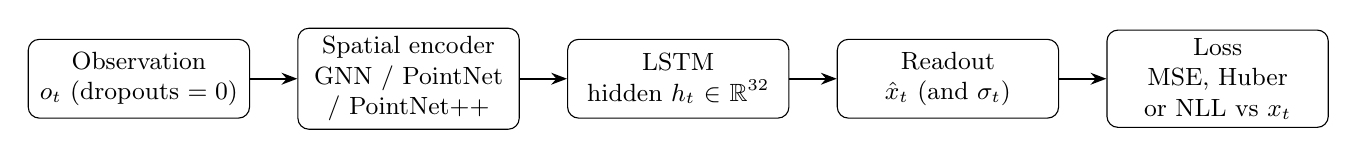
\begin{tikzpicture}[
  box/.style={draw, rounded corners, align=center, font=\small, inner sep=3pt, text width=2.6cm, minimum height=1.0cm},
  arr/.style={-{Stealth[length=2mm]}, thick}]
\node[box] (o) {Observation\\$o_t$ (dropouts $=0$)};
\node[box, right=0.6cm of o] (enc) {Spatial encoder\\GNN / PointNet / PointNet++};
\node[box, right=0.6cm of enc] (lstm) {LSTM\\hidden $h_t\in\mathbb{R}^{32}$};
\node[box, right=0.6cm of lstm] (out) {Readout\\$\hat x_t$ (and $\sigma_t$)};
\node[box, right=0.6cm of out] (loss) {Loss\\MSE, Huber or NLL vs $x_t$};
\draw[arr] (o) -- (enc);
\draw[arr] (enc) -- (lstm);
\draw[arr] (lstm) -- (out);
\draw[arr] (out) -- (loss);
\end{tikzpicture}
\caption{Observer data flow at one step. Only the encoder differs between architectures. Neural observers receive $o_t$ with dropouts encoded as zero; the ridge baseline also receives $m_t$.}
\label{fig:pipeline}
\end{figure*}

\textbf{Two-layer GNN.} With $\tilde A=A+I$, $\tilde D=\operatorname{diag}(\tilde A\mathbf 1)$ and $\hat A=\tilde D^{-1/2}\tilde A\tilde D^{-1/2}$, the layers are $H^{(l+1)}=\operatorname{ReLU}(\hat AH^{(l)}W^{(l)}+\mathbf 1 b^{(l)\top})$ for $l\in\{0,1\}$, with dense $W^{(l)}\in\mathbb{R}^{16\times 16}$. The first layer produces $H^{(1)}$ and the second $H^{(2)}$, a two-hop receptive field.

\textbf{Diagonal-gain GNN.} The form $\operatorname{diag}(W)\hat AH$ is implemented as a learnable diagonal gain on the left, $H^{(l+1)}=\operatorname{ReLU}(\operatorname{diag}(w^{(l)})\hat AH^{(l)}\Theta^{(l)}+\mathbf 1 b^{(l)\top})$ with $w^{(l)}\in\mathbb{R}^6$, $\Theta^{(l)}$ dense and $w^{(l)}$ initialized at one.

\textbf{Controls.} The four-layer GNN has four graph-convolution layers. The random-topology GNN uses a random symmetric graph with the same six edges. PointNet applies a shared MLP to each node's reading and a symmetric max over nodes; the max discards which tank produced which reading. We therefore also report PointNet with node identity, where each node input carries a one-hot node index. PointNet++ adds a local max over each closed neighbourhood before a global max. The parameter-matched PointNet widens its layers to 32 units. The Huber-loss control uses Huber loss with $\delta=0.5$ in place of the squared error.

\begin{table}[t]
\centering
\caption{Total trainable parameters.}
\label{tab:params_count}
\small
\begin{tabular}{lc}
\toprule
Model & Parameters \\
\midrule
Two-layer GNN (and Huber-loss GNN) & 10{,}526 \\
Four-layer GNN & 11{,}070 \\
Random-topology GNN & 10{,}526 \\
Diagonal-gain GNN & 10{,}538 \\
PointNet & 8{,}606 \\
PointNet with node identity & 8{,}702 \\
PointNet, parameter-matched & 10{,}590 \\
PointNet++ & 8{,}606 \\
Probabilistic GNN & 10{,}724 \\
\bottomrule
\end{tabular}
\end{table}

\subsection{Experimental protocol}
\label{sec:protocol}

Each run trains for 500 epochs with Adam (learning rate $10^{-3}$) on batches of 16 trajectories of length 64, with $p_{\text{event}}=0.08$. Every configuration is trained with ten seeds (0 to 9). Each trained model is evaluated on three independent test sets generated from seeds $777$, $888$ and $999$, each with 1{,}000 trajectories that include the recorded events.

Training variability (standard deviation over training seeds of the per-seed mean over test sets) and test-sampling variability (standard deviation over the three test sets for a fixed model) are reported separately. Paired comparisons share the training seed, use a two-sided paired $t$-test and a 95\% $t$ interval over the ten differences. No correction is made for multiple comparisons. The linear baseline has no training seeds: it is one ridge fit, so its spread is over the three test sets only.

\subsection{Training variability dominates}

For every neural configuration, the test-set standard deviation for a fixed model is between $0.0005$ and $0.0017$ in MSE, while the training-seed standard deviation is between $0.034$ and $0.123$. Differences between configurations are therefore estimated from the training seeds.

\subsection{Architectures and controls}

\begin{table*}[t]
\centering
\caption{Estimation error by encoder and control (ten training seeds, three test sets each).}
\label{tab:archs}
\small
\begin{tabular}{lcccc}
\toprule
Model & MSE (mean $\pm$ sd over seeds) & Tank MSE & Junction MSE & Seeds lower than two-layer GNN \\
\midrule
Two-layer GNN & $0.326\pm0.105$ & $0.161$ & $0.408$ & --- \\
Four-layer GNN & $0.262\pm0.057$ & $0.137$ & $0.325$ & 7 of 10 \\
Random-topology GNN & $0.311\pm0.101$ & $0.151$ & $0.391$ & 8 of 10 \\
Huber-loss GNN & $0.331\pm0.123$ & $0.140$ & $0.427$ & 4 of 10 \\
PointNet & $0.219\pm0.040$ & $0.123$ & $0.268$ & 10 of 10 \\
PointNet with node identity & $0.231\pm0.043$ & $0.130$ & $0.282$ & 8 of 10 \\
PointNet, parameter-matched & $0.212\pm0.084$ & $0.128$ & $0.253$ & 8 of 10 \\
PointNet++ & $0.228\pm0.054$ & $0.132$ & $0.275$ & 8 of 10 \\
\bottomrule
\end{tabular}
\end{table*}

\begin{figure}[t]
\centering
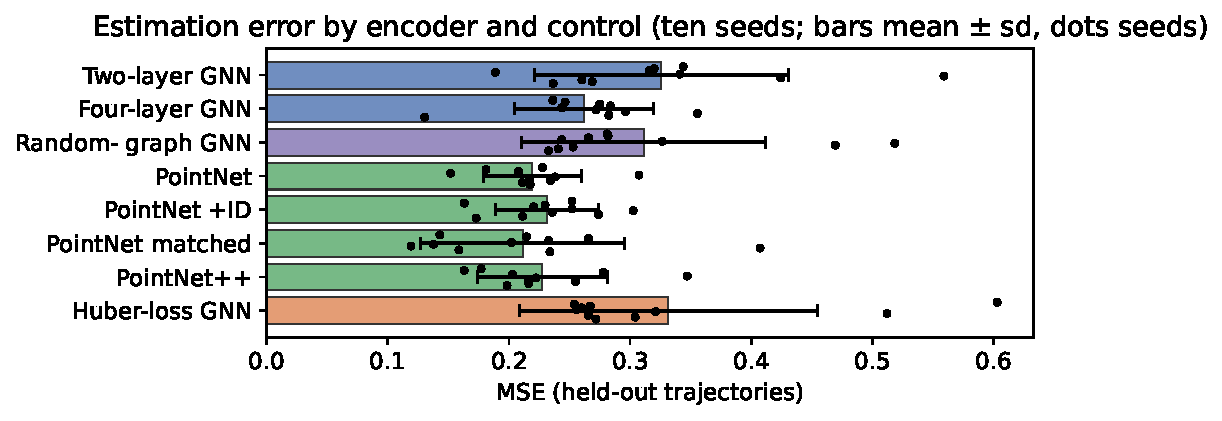
\includegraphics[width=\linewidth]{fig_architectures.pdf}
\caption{Estimation error by encoder and control over ten training seeds.}
\label{fig:arch}
\end{figure}

Plain PointNet is lower than the two-layer GNN on all ten seeds ($-0.106$, 95\% CI $[-0.176,-0.037]$, $p=0.007$). Adding node identity does not improve PointNet ($+0.012$ relative to plain PointNet, 95\% CI $[-0.018,0.042]$, $p=0.39$), so missing node labels are not what limits it here. The parameter-matched PointNet is lower than the GNN on eight of ten seeds, with a CI that includes zero ($p=0.058$). The random-topology control is not significantly different from the GNN, so the actual graph does not clearly help in this benchmark.

\begin{figure}[t]
\centering
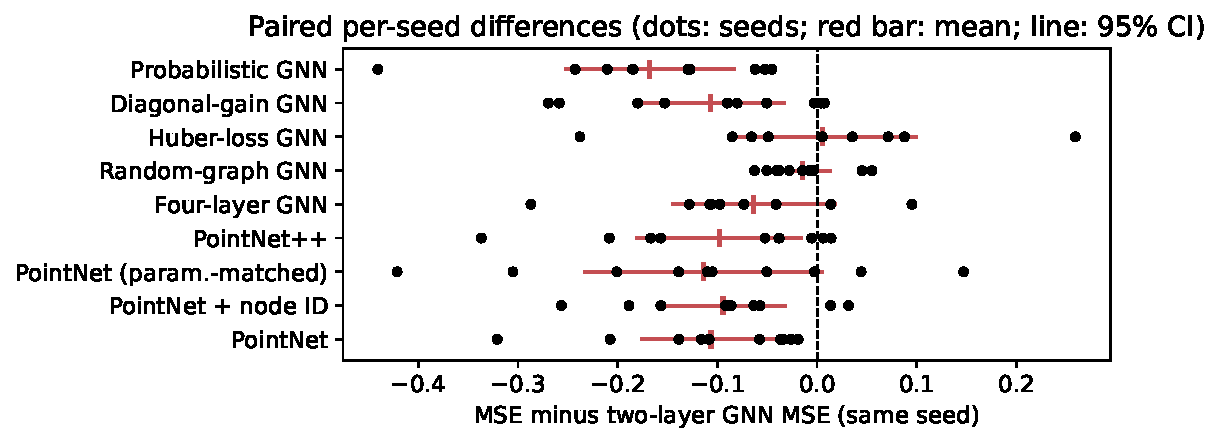
\includegraphics[width=\linewidth]{fig_paired.pdf}
\caption{Paired per-seed differences from the two-layer GNN with 95\% confidence intervals.}
\label{fig:paired}
\end{figure}

\subsection{Dense and diagonal gains, homogeneous and heterogeneous pipes}
\label{sec:hetero}

On homogeneous pipes the diagonal-gain GNN is lower than the dense GNN ($-0.107$, 95\% CI $[-0.182,-0.033]$, lower on eight of ten seeds). On heterogeneous pipes the difference is $-0.056$ ($p=0.16$, not significant). Heterogeneous conductance does not significantly change either encoder. Table~\ref{tab:dense} gives the values.

\begin{table}[t]
\centering
\caption{Dense and diagonal-gain GNN with homogeneous and heterogeneous conductance (ten seeds).}
\label{tab:dense}
\small
\resizebox{\linewidth}{!}{%
\begin{tabular}{llccc}
\toprule
Encoder & Pipes & MSE & Tank MSE & Junction MSE \\
\midrule
Dense $W$ & homogeneous & $0.326\pm0.105$ & $0.161$ & $0.408$ \\
Dense $W$ & heterogeneous & $0.301\pm0.080$ & $0.146$ & $0.379$ \\
Diagonal $w$ & homogeneous & $0.219\pm0.056$ & $0.115$ & $0.270$ \\
Diagonal $w$ & heterogeneous & $0.246\pm0.081$ & $0.125$ & $0.306$ \\
\bottomrule
\end{tabular}}
\end{table}

The diagonal-gain GNN and the parameter-matched PointNet are not significantly different in this test (difference $+0.007$, 95\% CI $[-0.057,+0.071]$, $p=0.81$). We name no deterministic winner.

\section{Probabilistic observer, calibration and event detection}

\subsection{Probabilistic observer and the source of its gain}
\label{sec:prob}

The probabilistic GNN has MSE $0.158\pm0.034$ and beats the two-layer GNN on all ten paired seeds ($-0.168$, 95\% CI $[-0.252,-0.084]$, $p=0.0015$). Table~\ref{tab:controls} gives the controls that separate possible sources of the gain.

\begin{table}[t]
\centering
\caption{Controls for the probabilistic gain (ten seeds, three test sets each).}
\label{tab:controls}
\small
\setlength{\tabcolsep}{3pt}
\resizebox{\linewidth}{!}{%
\begin{tabular}{p{4.2cm}ccc}
\toprule
Model & MSE & Difference from probabilistic GNN & $p$ \\
\midrule
Plain GNN (MSE) & $0.326\pm0.105$ & $+0.168$ (95\% CI $[+0.084,+0.252]$) & 0.0015 \\
Isolated variance head: mean weighted by detached variance & $0.188\pm0.064$ & $+0.030$ (95\% CI $[-0.026,+0.086]$) & 0.26 \\
Two-stage weighting: MSE weighted by a frozen separate variance model & $0.540\pm0.167$ & $+0.382$ (95\% CI $[+0.250,+0.514]$) & 0.0001 \\
Huber-loss GNN & $0.331\pm0.123$ & $+0.173$ (95\% CI $[+0.081,+0.266]$) & 0.002 \\
\bottomrule
\end{tabular}}
\end{table}

\begin{figure}[t]
\centering
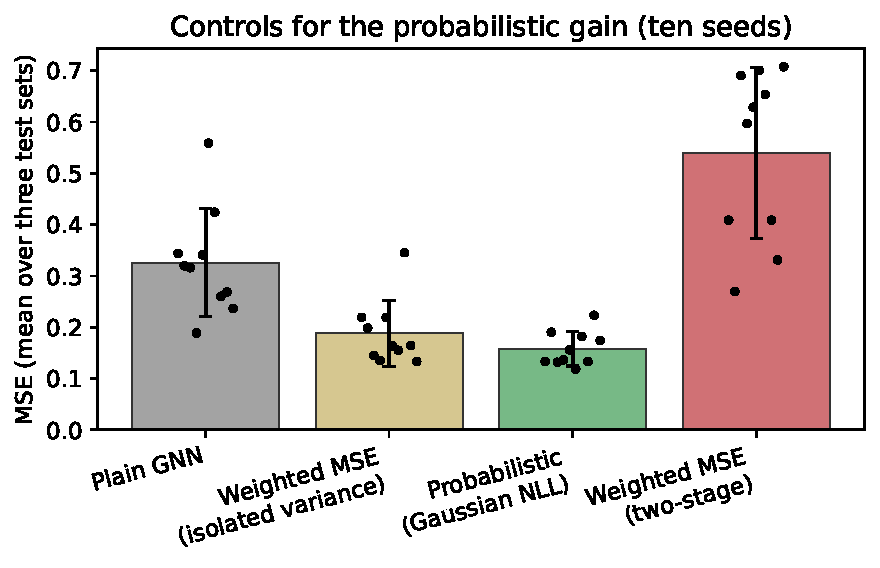
\includegraphics[width=0.7\linewidth]{fig_controls.pdf}
\caption{Controls for the probabilistic gain over ten seeds.}
\label{fig:controls}
\end{figure}

The isolated-variance control keeps most of the gain. Its mean loss is weighted per sample by the detached variance and its variance head sees only detached features, so the variance can shape the mean gradient but cannot change the encoder through the variance loss. It recovers $0.138$ of the $0.168$ improvement over the plain GNN. The remaining $0.030$ is not significant. The ablation results are consistent with adaptive per-sample loss weighting explaining most of the observed improvement. The isolated-variance control still learns the variance jointly with the mean, so it removes one gradient pathway, not all influence of uncertainty learning. The two-stage control, which uses weights from a separate frozen model, is much worse than the plain GNN. The weights only help when mean and variance are learned together; the separate weights appear to destabilize training. The Huber-loss control shows that down-weighting large errors without a variance model does not help.

\textbf{Calibration.} Empirical coverage at nominal levels 50, 80, 90, 95 and 99\% is $0.623$, $0.867$, $0.925$, $0.950$ and $0.973$ (standard deviation over seeds $0.046$ to $0.004$). Intervals are conservative at lower levels and close to nominal at 90\%, 95\% and 99\%. At the 95\% level, coverage is $0.93$ for each tank and $0.96$ for each junction. It is $0.98$ at calm steps but only $0.89$ at event-active steps, so intervals are too narrow during disturbances. The probabilistic model's held-out negative log-likelihood is $0.291\pm0.127$ per value.

\begin{figure*}[t]
\centering
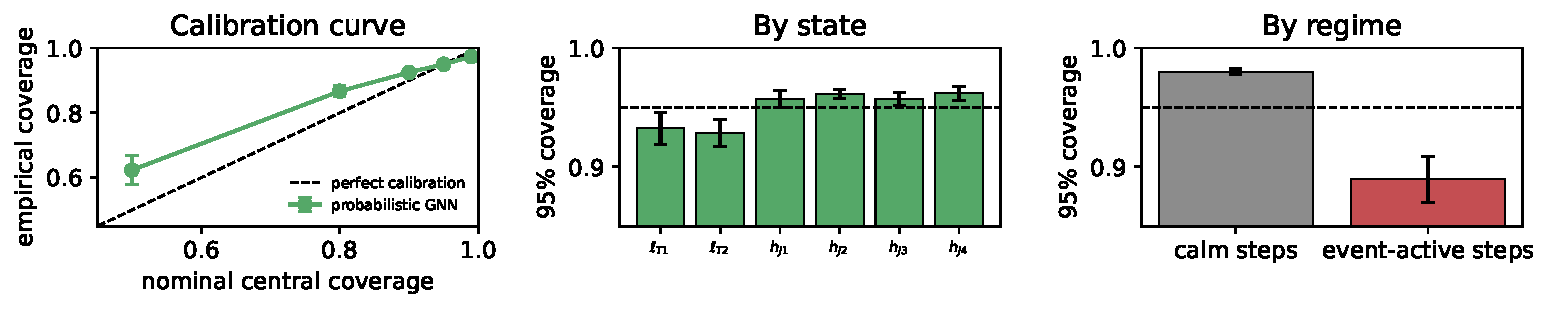
\includegraphics[width=\textwidth]{fig_calibration.pdf}
\caption{Left: calibration curve. Centre: 95\% coverage by state. Right: 95\% coverage at calm and event-active steps.}
\label{fig:calib}
\end{figure*}

\subsection{Calibration by event type and in the weakly observable direction}
\label{sec:calibevents}

We retrained the probabilistic GNN for five seeds (seeds 0--4 of the ten used elsewhere) and split coverage, interval width and realised error by event type (Fig.~\ref{fig:calibevents}). Coverage of the nominal 95\% interval is $0.982$ at calm steps and $0.975$ during sensor dropouts, but only $0.826$ during pump trips and $0.859$ during demand spikes (standard deviation over seeds $0.065$ and $0.011$). Over the same steps the realised RMSE rises from $0.30$ at calm steps to $0.50$ at pump trips and $0.64$ at demand spikes, while the mean predicted standard deviation barely moves ($0.34$ at calm steps, $0.38$ at pump trips, $0.34$ at demand spikes). The shortfall in the 88.9\% event-active coverage therefore comes from pump trips and demand spikes and it arises because the predicted uncertainty is close to constant across regimes: the model does not widen its intervals when the error grows. This is consistent with the weak predictive-sd AUCs in Table~\ref{tab:events}.

For the J2-minus-J4 direction, taking the per-state predicted variances as independent (an approximation), the mean predicted standard deviation is $0.45$ and the realised RMSE is $0.265$, which equals the prior-only level ($\sqrt{0.0695}=0.264$). The 95\% intervals cover $96.8\%$ of the values in that direction and are about $1.7$ times wider than the realised error. Coverage there is adequate because the intervals are conservative, not because the model has identified how little the sensors reveal about the mode.

\begin{figure}[t]
\centering
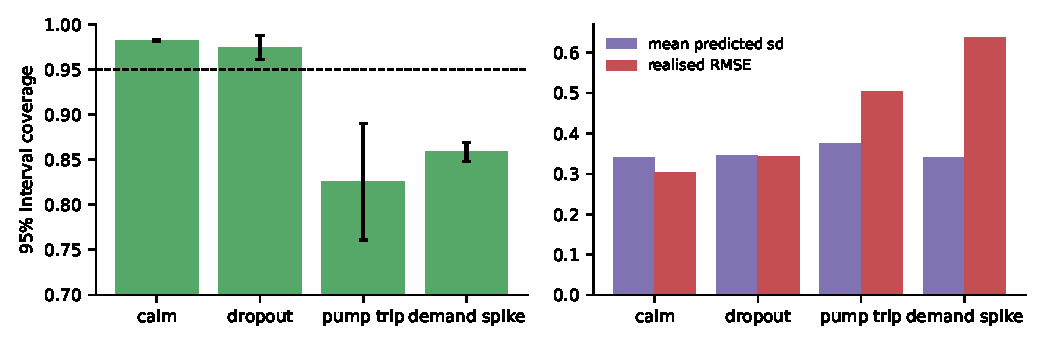
\includegraphics[width=\linewidth]{fig_calib_events.pdf}
\caption{Probabilistic GNN by event type (five seeds, error bars are one standard deviation over seeds). Left: coverage of the nominal 95\% interval. Right: mean predicted standard deviation and realised RMSE.}
\label{fig:calibevents}
\end{figure}

\subsection{Detecting disturbance events}
\label{sec:events}

We score event-active steps against calm steps with ROC AUC, where $0.5$ is chance, for two scores that use only sensor readings. The observer score is the absolute difference between each reported tank reading and the observer's estimate, averaged over reported tanks. The linear score is the one-step-ahead innovation, the absolute difference between each reported tank reading and its prediction from the previous six steps, averaged over reported tanks.

Sensor dropouts are excluded from these claims. A masked tank changes the average, because the score is taken over fewer readings. The dropout AUCs we first computed were confounded by this and are not reported as detection results. The dropout case needs a score that does not depend on the number of reporting tanks.

Table~\ref{tab:events} gives the remaining results. The observer's residual detects pump trips well (AUC $0.93$), because a tank that stops being refilled falls away from its estimate. It is near chance for demand spikes ($0.56$). The predicted standard deviation is weaker for both events. The linear innovation is below chance for demand spikes, so in this experiment the linear innovation score is inversely associated with demand-spike labels. The mechanism is not established; changes in the residual distribution or in the score direction could contribute.

\begin{table}[t]
\centering
\caption{ROC AUC for event-active steps, by event type (calm steps as negatives).}
\label{tab:events}
\small
\setlength{\tabcolsep}{3pt}
\resizebox{\linewidth}{!}{%
\begin{tabular}{lcc}
\toprule
Score & Pump trip & Demand spike \\
\midrule
Observer residual (probabilistic GNN, ten seeds) & $0.929\pm0.014$ & $0.564\pm0.036$ \\
Predicted standard deviation (probabilistic GNN, ten seeds) & $0.681\pm0.041$ & $0.524\pm0.012$ \\
One-step innovation (linear, one fit) & $0.485$ & $0.382$ \\
\bottomrule
\end{tabular}}
\end{table}

Events cover about one third of steps here, so these are benchmark measurements, not rates for rarer events.

\section{Filter versus smoother by regime}
\label{sec:smoother}

Under calm conditions the RTS smoother is about four times more accurate than the filter (ratio $0.23$--$0.27$) (Table~\ref{tab:smoother}), as expected for a correctly specified linear Gaussian model. Under disturbance events it is about $2\%$ less accurate (ratio $1.02$) and with $Q$ taken from calm data it is $33\%$ less accurate (ratio $1.33$). This reversal should not be read as a property of smoothing. An exact conditional-mean smoother for a correctly specified model and the matching evaluation distribution cannot have a higher expected squared error than its own filter. The reversal therefore points to model mismatch (here, a single effective $Q$ for what is really a two-regime disturbance process), finite-sample evaluation, or both: it is larger when $Q$ is calibrated on calm data and the evaluation is on events (ratio $1.33$) than when $Q$ comes from event data (ratio $1.02$). A plausible but untested mechanism is that the backward pass propagates an unmodelled shock to earlier steps.

\begin{table}[t]
\centering
\caption{Kalman filter and RTS smoother by regime (300 trajectories each; events at rate $0.08$).}
\label{tab:smoother}
\small
\resizebox{\linewidth}{!}{%
\begin{tabular}{lccc}
\toprule
Regime and $Q$ calibration & Filter MSE & Smoother MSE & Ratio \\
\midrule
Calm, $Q$ from calm data & $0.00374$ & $0.00085$ & $0.23$ \\
Calm, $Q$ from event data & $0.00412$ & $0.00112$ & $0.27$ \\
Events, $Q$ from event data & $0.07171$ & $0.07331$ & $1.02$ \\
Events, $Q$ from calm data & $0.09707$ & $0.12942$ & $1.33$ \\
\bottomrule
\end{tabular}}
\end{table}

\footnotesize
\section{Hydraulic simulation check}

This appendix repeats the estimator comparison on data from a hydraulic simulation with the EPANET engine of the same graph. It addresses the objection that the benchmark is not a hydraulic model; it is still a simulation, uses homogeneous pipes and no real measurements, and does not replace field validation.

\textbf{Model.} The network is built with WNTR~\cite{klise2017} and simulated with the EPANET 2.2 hydraulic engine (WNTR's \texttt{EpanetSimulator}), which generated all the data used below. As a check, an earlier version of the experiment generated the data with WNTR's own Python solver instead: the heads agree to about $2\times10^{-5}$~m on test trajectories and the estimator MSEs agree to the third decimal (GRU $0.339$ against $0.339$, supervised IMM $0.352$ against $0.353$, label-free IMM $0.402$ against $0.402$). It has the benchmark's graph: tank $T_1$ on junction $J_1$, tank $T_2$ on $J_3$ and the ring $J_1$--$J_2$--$J_3$--$J_4$, with identical pipes (diameter $0.25$~m, length $600$~m, Hazen--Williams coefficient $100$). The tanks are cylinders of diameter $14$~m, start at a level of $8$~m and are each fed from a fixed-head reservoir (head $9$~m) through a supply pipe, so the inflow depends on the head difference to the tank (a hydraulic analogue of the proportional pump controller). Every junction has a base demand of $0.010$~m$^3$/s with the diurnal pattern $1+0.5\sin(2\pi t/48)$ and Gaussian noise of standard deviation $0.004$~m$^3$/s at each 30-minute step. Events follow the benchmark's process (one at a time, six steps, probability $0.08$ per step when none is active, type and location uniform): a pump trip closes the supply pipe of one tank (EPANET time controls), a demand spike multiplies the demand of one junction by four, and a dropout removes one tank reading. The state is the vector of node heads (tank level plus elevation $0$, junction heads); the observations are the two tank heads with noise of standard deviation $0.03$~m. The start is not exactly fixed here, because the initial junction heads depend on the first demand draw (spread up to $0.46$~m); the filters use the mean and covariance of the training start states.

\textbf{Protocol.} Training uses $2000$ trajectories (the hidden junction heads, and for supervised identification the regime labels, as for the benchmark) and testing $900$ trajectories, with only tank readings and masks as inputs at test time; errors are over steps $1$--$63$. The estimators are the benchmark's, with no tuning for this system: a ridge regression on a $64$-step window (penalty $0.01$ chosen on a validation set); a GRU with $64$ hidden units (three seeds, the configuration selected on the benchmark); a single-regime Kalman filter whose transition matrix, forcing and covariance are least-squares fits to the training states; an IMM with the seven regimes identified by regression with regime labels; and an IMM identified without labels (k-means with hard EM, $K=9$, three seeds). Table~\ref{tab:hydraulic} gives the MSE in m$^2$ over all states and in the $J_2$--$J_4$ direction.

\textbf{Results.} (i) The unobservable direction is reproduced: the error in the $J_2$--$J_4$ direction is $0.050$ without any sensor and between $0.050$ and $0.053$ for every estimator, so no estimator improves on the prior-only level, as on the synthetic benchmark. (ii) The GRU ($0.339$) is $31\%$ below the ridge regression ($0.489$) and $28\%$ below the identified Kalman filter ($0.470$). (iii) The IMMs do not beat the GRU here: the supervised IMM reaches $0.352$ and the label-free IMM $0.402$ (range $0.396$--$0.409$ over three seeds), above the GRU's $0.339$. The IMM's lead over the networks on the synthetic benchmark therefore does not carry over to this system, in line with the nonlinear-flow and mismatch results: the regime models are linear fits to nonlinear hydraulics, and the identified switching structure is a rough fit (the label-free groups represent $5$--$6$ of the seven true regimes, with training purity $0.86$--$0.87$ by majority vote). The orderings among the network, ridge and no-sensor estimators and the prior-level error in the unobservable direction are the findings that survive this change of simulator.

\textbf{Limitations.} The estimator comparison above is a single hydraulic configuration with homogeneous pipes (the placement study below uses $15$ configurations); no hyper-parameters were tuned for it; the IMM structure (seven regimes, six-state linear model) was inherited from the benchmark; the sensor-only identification of the main text was not repeated; and the shifts of Appendix~B were not repeated. The simulation is reproducible with \texttt{epanet\_simulator.py} and \texttt{hydraulic\_estimators.py}.

\begin{table}[t]
\centering
\caption{Estimators on the hydraulic simulation.}
\label{tab:hydraulic}
\small
\setlength{\tabcolsep}{3pt}
\resizebox{\linewidth}{!}{%
\begin{tabular}{lcc}
\toprule
Estimator & MSE (m$^2$) & $J_2$--$J_4$ (m$^2$) \\
\midrule
No sensors (time only) & $0.779$ & $0.050$ \\
Ridge, 64 steps & $0.489$ & $0.050$ \\
Kalman filter, identified & $0.470$ & $0.050$ \\
IMM, supervised identification & $0.352$ & $0.051$ \\
IMM, label-free identification & $0.402 [0.396, 0.409]$ & $0.053$ \\
GRU & $0.339 [0.337, 0.340]$ & $0.050$ \\
\bottomrule
\end{tabular}}
\end{table}



\subsection*{Placement rules on the hydraulic simulation}
The placement rules of Appendix~I were evaluated on EPANET-engine simulations of the same graph in $15$ hydraulic configurations (\texttt{placement.py hydraulic}): three with homogeneous pipes and $12$ with heterogeneous pipe diameters (factors in $[0.8,1.25]$), each with its own Hazen--Williams roughness ($80$--$140$) and pipe length ($400$--$900$~m), and with the events of this appendix (pump trips, demand spikes, dropouts). Each configuration has $1000$ training and $300$ test trajectories. One or two extra junction sensors (noise $0.03$~m, never dropped) were chosen by the six rules of Appendix~I, computed either from the nominal homogeneous linear model of the benchmark (no knowledge of the configuration) or from a linear model fitted to the configuration's training states ($x_{t+1}=Ax_t+c_0+c_1\sin+c_2\cos$ by least squares). The realised error is that of a ridge regression on a six-step window of the readings (tanks, masks and the extra sensors) predicting the four junction heads, which is independent of the rules; Table~\ref{tab:placement_hyd} gives the mean error along $(J_2-J_4)/\sqrt2$ relative to the best set of each configuration. The numbers are from Linux (Ubuntu under WSL), where five reruns gave identical output; Windows runs differed (below).

With two sensors:
\begin{itemize}
\item the weak-direction posterior rule chooses the pair $\{J_2,J_4\}$ in all $15$ configurations with the nominal model and in $14$ with the fitted model. This pair is the best set for the weak-direction error and for the total error in all $15$ configurations; its weak-direction error is $0.0008$ against $0.0385$ for the tank-only ridge regression (mean over configurations);
\item the symmetry rule chooses the same pair in all $15$ configurations, and the Gramian-trace rule chooses it in all configurations with the nominal model but in only $10$ of $15$ with the fitted model;
\item the Gramian-eigenvalue and posterior-trace rules, computed from the nominal model, choose in every configuration a pair that does not contain both $J_2$ and $J_4$, and have $20.6$ times the weak-direction error of the best set (random choice: $20.7$); with the fitted model the Gramian-eigenvalue and trace rules are still $10$--$13$ times worse on average and the posterior-trace rule $1.8$ times worse.
\end{itemize}
With one sensor the best set for the weak direction is $J_2$ or $J_4$ in $15$ of $15$ configurations, which the weak-direction rule chooses with the nominal model (ratio $1.08$ against $1.11$ for random choice), but the best set for the total error is a central junction ($J_1$ or $J_3$) in $15$ of $15$ configurations, so targeting the weak direction costs total error (ratio $1.45$ against $1.29$ for random choice).

On this simulation, in these $15$ configurations, the rules that name the weak direction, or the symmetry that produces it, choose the pair $\{J_2,J_4\}$, and the generic Gramian and posterior criteria do not when they are computed from a model that does not break the symmetry; this is consistent with the linear-Gaussian comparison but is a check on a small choice set (six pairs), not a general confirmation of the rankings. Two limits remain. With two sensors on $J_2$ and $J_4$ the ridge regression reads the difference almost directly (its error is near the sensor noise variance $9\times10^{-4}$), so the large ratios reflect how much the other pairs lose and the test is of the choice of pair, not of a predicted size of the reduction; and the study uses one graph with four candidate junctions, one estimator, and heterogeneity only through pipe diameters.

\begin{table*}[t]
\centering
\caption{Placement rules on EPANET-engine simulations: weak-direction error relative to the best set.}
\label{tab:placement_hyd}
\small
\resizebox{\linewidth}{!}{%
\begin{tabular}{lcccccc}
\toprule
Setting & Random & Symmetry & Gramian $\lambda_{\min}$ & Gramian trace & Posterior trace & Weak-direction posterior \\
\midrule
1 sensor, design on nominal model & $1.11$ & $1.08$ & $1.08$ & $1.08$ & $1.08$ & $1.08$ \\
1 sensor, design on fitted model & $1.11$ & $1.08$ & $1.02$ & $1.14$ & $1.01$ & $1.01$ \\
2 sensors, design on nominal model & $20.72$ & $1.00$ & $20.57$ & $1.00$ & $20.57$ & $1.00$ \\
2 sensors, design on fitted model & $20.72$ & $1.00$ & $12.81$ & $10.18$ & $1.83$ & $1.06$ \\
\bottomrule
\end{tabular}}
\end{table*}

\textbf{Reproducibility.} The Linux numbers of Table~\ref{tab:placement_hyd} were repeated five times with identical output (\texttt{hydraulic\_repeats\_summary.py}). The first run, made on Windows, and two later Windows reruns gave different values for the rules that depend on the fitted model (Table~\ref{tab:hydraulic_repeats}), and the Windows runs also differ from each other, whereas the Linux runs do not. We have not isolated the cause of either difference. The differences do not touch the realised best sets: in every configuration of every run the best pair is $\{J_2,J_4\}$ for both objectives, and with one sensor the best junction is $J_2$ or $J_4$ for the weak direction and $J_1$ or $J_3$ for the total error. The symmetry rule chooses $\{J_2,J_4\}$ in all $15$ configurations of every run. The rules that depend on the fitted model change most: the posterior-trace rule has a ratio of $1.83$ on Linux and $1.75, 3.29, 3.30$ on Windows, and the weak-direction posterior rule chooses the pair in $14$ configurations on Linux and in $15, 14, 14$ on Windows, with a ratio of at most $1.06$ in every run.

\begin{table}[t]
\centering
\caption{The hydraulic placement experiment in two computing environments (two sensors, design on the fitted model).}
\label{tab:hydraulic_repeats}
\small
\setlength{\tabcolsep}{3pt}
\resizebox{\linewidth}{!}{%
\begin{tabular}{lcccccc}
\toprule
 & \multicolumn{2}{c}{Ratio to best set} & \multicolumn{4}{c}{Configs choosing $\{J_2,J_4\}$ (of 15)} \\
\cmidrule(lr){2-3}\cmidrule(lr){4-7}
Run & Posterior trace & Weak-direction posterior & Weak-direction posterior & Posterior trace & Gramian trace & Gramian $\lambda_{\min}$ \\
\midrule
Windows, first run & $1.75$ & $1.00$ & 15 & 14 & 9 & 6 \\
Windows, rerun 1 & $3.29$ & $1.06$ & 14 & 12 & 9 & 5 \\
Windows, rerun 2 & $3.30$ & $1.06$ & 14 & 12 & 9 & 5 \\
Linux, five reruns (identical) & $1.83$ & $1.06$ & 14 & 13 & 10 & 4 \\
\bottomrule
\end{tabular}}
\end{table}

\section{Proofs of Propositions~\ref{prop:scaling}--\ref{prop:orbit}}
\label{app:proof}

\begin{proof} Throughout, $T\ge6$ and $\varepsilon$ is small; $M(\varepsilon)=M_T(\varepsilon)$ is a polynomial in $\varepsilon$, $M(0)=M_0$ has rank five and $M_0v=0$, so $M_0$ is injective on $v^\perp$ and $\sigma_*=\sigma_{\min}(M_0|_{v^\perp})>0$.
\emph{(a)} If $A_1v=\mu v$ then $A(\varepsilon)v=(\lambda+\varepsilon\mu)v$ and $CA(\varepsilon)^jv=(\lambda+\varepsilon\mu)^jCv=0$ for all $j$.
\emph{(b), first claim.} $M(\varepsilon)v=\varepsilon c+O(\varepsilon^2)$ since $M_0v=0$. Let $y_\varepsilon\perp v$ minimise $\|M(\varepsilon)(v+y)\|$. Comparing with $y=0$ gives $\|M(\varepsilon)(v+y_\varepsilon)\|\le\|M(\varepsilon)v\|=O(\varepsilon)$, hence $\sigma_*\|y_\varepsilon\|-O(\varepsilon)\|y_\varepsilon\|-O(\varepsilon)\le O(\varepsilon)$ and $\|y_\varepsilon\|=O(\varepsilon)$. Then $M(\varepsilon)(v+y_\varepsilon)=M_0y_\varepsilon+\varepsilon c+O(\varepsilon^2)$, and applying $\Pi$ (which annihilates $M_0y_\varepsilon$) gives $\|M(\varepsilon)(v+y_\varepsilon)\|\ge\varepsilon\|\Pi c\|-O(\varepsilon^2)$. Conversely $y=-\varepsilon M_0^{+}c$ gives $\|M(\varepsilon)(v+y)\|\le\varepsilon\|\Pi c\|+O(\varepsilon^2)$. So $s(\varepsilon)=\varepsilon^2\|\Pi c\|^2+O(\varepsilon^3)$.
\emph{(b), second claim.} In the basis $(v,v^\perp)$ write $W=W_T(\varepsilon)=\begin{bmatrix}w_{vv}&w_{vr}^\top\\w_{vr}&W_{rr}\end{bmatrix}$. By Weyl's inequality and continuity, $W_{rr}(\varepsilon)\succeq\gamma I$ for $|\varepsilon|\le\varepsilon_0$, with $\gamma=\sigma_*^2/2$ ($W_{rr}(0)=(M_0|_{v^\perp})^\top M_0|_{v^\perp}\succeq\sigma_*^2I$), and $w_{vr}=(Wv)_{v^\perp}=M_{v^\perp}^\top M v=O(\varepsilon)$. Put $q=W_{rr}^{-1}w_{vr}$, so $\|q\|\le\|w_{vr}\|/\gamma=O(\varepsilon)$, and $s=w_{vv}-w_{vr}^\top W_{rr}^{-1}w_{vr}$, which is the quantity minimised in (b) (minimise $\|M(v+y)\|^2=w_{vv}+2w_{vr}^\top y+y^\top W_{rr}y$ over $y$). For $x=(a,y)$, $x^\top Wx=a^2s+(y+aq)^\top W_{rr}(y+aq)$. \emph{Upper bound:} $x=(1,-q)/\sqrt{1+\|q\|^2}$ gives $\lambda_{\min}\le s/(1+\|q\|^2)$. \emph{Lower bound:} let $x$ be a unit vector with $x^\top Wx=\lambda_{\min}$, $t=|a|$. If $\|y\|\ge2t\|q\|$ then $\|y+aq\|\ge\|y\|/2$, so $x^\top Wx\ge t^2s+\tfrac{\gamma}{4}(1-t^2)\ge\min(s,\gamma/4)=s$ for $s\le\gamma/4$. Otherwise $1-t^2=\|y\|^2<4t^2\|q\|^2$, so $t^2>1/(1+4\|q\|^2)$ and $x^\top Wx\ge t^2s\ge s/(1+4\|q\|^2)$. In both cases $\lambda_{\min}\ge s/(1+4\|q\|^2)$, so $\lambda_{\min}=s(1+O(\varepsilon^2))$.
\emph{(c)} With $H=P_0^{-1}+W/\sigma_v^2$ and the Schur complement with respect to $v$, $v^\top H^{-1}v=\big(1/p+\delta/\sigma_v^2\big)^{-1}$ with $\delta=w_{vv}-w_{vr}^\top(W_{rr}+\sigma_v^2p^{-1}I)^{-1}w_{vr}$. Since $(W_{rr}+\sigma_v^2p^{-1}I)^{-1}\preceq W_{rr}^{-1}$, $s\le\delta\le w_{vv}$, and the reduction is $(p\delta/\sigma_v^2)/(1+p\delta/\sigma_v^2)$. Here $s=\varepsilon^2\|\Pi c\|^2(1+O(\varepsilon))$ and $w_{vv}=\|M(\varepsilon)v\|^2=\varepsilon^2\|c\|^2+O(\varepsilon^3)$, which gives $\kappa_1\varepsilon^2\le$ reduction $\le\kappa_2\varepsilon^2$.
\emph{(d)} From the incidence matrix, $N^\top v=2^{-1/2}(0,0,-1,1,1,-1)^\top$, so $A_1v\propto(0,0,u_6-u_3,\,u_3+u_4,\,u_5-u_4,\,-u_5-u_6)^\top$, which is proportional to $v$ if and only if $u_3=u_6$ and $u_4=u_5$. The vector $c$ is linear in $u$ and vanishes for such $u$ (then $A_1v\in\operatorname{span}(v)$ and every $CA_0^{\,m}A_1v=0$), hence $c(u)=c(u_a)$ with $u_a=(0,0,a,b,-b,-a)$, $a=(u_3-u_6)/2$, $b=(u_4-u_5)/2$ the mirror-antisymmetric part, and $\|\Pi c\|^2=(a,b)\,G\,(a,b)^\top$ with a symmetric $2\times2$ matrix $G$. We computed $G$ in exact rational arithmetic (\texttt{proposition1\_exact\_certificate.py}), with $\Pi$ built from the exact inverse of $B^\top M_0^\top M_0B$ for a basis $B$ of $v^\perp$. For $T=6$: $G_{11}=G_{22}=4.8481e-03$, $G_{12}=-4.2687e-03$, $\det G=5.2826e-06>0$; for $T=64$: $G_{11}=G_{22}=1.2348e-02$, $G_{12}=-4.2459e-03$, $\det G=1.3446e-04>0$. Both leading principal minors are positive, so $G$ is positive definite for these two horizons (values shown to four digits; the signs are those of the exact rational numbers).\end{proof}

\subsection*{Proofs of Propositions~\ref{prop:sym} and~\ref{prop:orbit}}
\emph{Proposition~\ref{prop:sym}(a).} Since every $g\in\mathcal G$ fixes the tank nodes, $C\Pi_g=C$, and since $L$, $E$ and (for a $\mathcal G$-invariant perturbation) the conductances are invariant, $A\Pi_g=\Pi_gA$. Hence $CA^j\Pi_g=C\Pi_gA^j=CA^j$ and for $x\in\ker P$, $CA^jx=|\mathcal G|^{-1}\sum_g CA^j\Pi_gx=CA^jPx=0$, so $V_0\subseteq N_0$.

\emph{Proposition~\ref{prop:sym}(b).} Write $W=W_T(\varepsilon)$ in the basis $(N_0,N_0^\perp)$ with blocks $W_{vv}$, $W_{vr}$, $W_{rr}$. As in the proof of Proposition~\ref{prop:scaling}, $M_T(\varepsilon)U=\varepsilon c+O(\varepsilon^2)$, $M_T(0)$ is injective on $N_0^\perp$ (by the definition of $N_0$), $W_{rr}\succeq\gamma I$ with $\gamma=\sigma_*^2/2$ for small $\varepsilon$ and $W_{vr}=O(\varepsilon)$. The Schur complement $S=W_{vv}-W_{vr}^\top W_{rr}^{-1}W_{vr}$ is the minimum, in the Loewner order, of $(U+Y)^\top W(U+Y)$ over $Y$ with columns in $N_0^\perp$ (equivalently of $\|M_T(\varepsilon)(U+Y)\|^2$), the minimiser $Y$ is $O(\varepsilon)$, and the argument of Proposition~\ref{prop:scaling}(b) gives $S=\varepsilon^2H(u)+O(\varepsilon^3)$. With $Q=W_{rr}^{-1}W_{vr}$ and $T_0=\begin{bmatrix}I&0\\Q&I\end{bmatrix}$ we have $W=T_0^\top\operatorname{diag}(S,W_{rr})T_0$, where $T_0=I+O(\varepsilon)$. By Ostrowski's theorem on congruence~\cite{horn2013}, $\lambda_i(W)=\theta_i\lambda_i(\operatorname{diag}(S,W_{rr}))$ with $\theta_i\in[\sigma_{\min}(T_0)^2,\sigma_{\max}(T_0)^2]=[1-O(\varepsilon),1+O(\varepsilon)]$. For small $\varepsilon$ the $d$ smallest eigenvalues of $\operatorname{diag}(S,W_{rr})$ are those of $S$, because $\lambda_{\max}(S)=O(\varepsilon^2)<\gamma$. Hence $\lambda_i(W)=\theta_i\lambda_i(S)$ with $\theta_i=1+O(\varepsilon)$, and by Weyl's inequality $\lambda_i(S)=\varepsilon^2\lambda_i(H(u))+O(\varepsilon^3)$, so $\lambda_i(W)=\varepsilon^2\lambda_i(H(u))+O(\varepsilon^3)$. This is an absolute error bound, so it also holds when $\lambda_i(H(u))=0$; the relative error is $O(\varepsilon)$ when $\lambda_i(H(u))>0$.

\emph{Proposition~\ref{prop:sym}(c).} Let $N_0=V_0$. The vector $c$ is linear in $u$. If $u=\bar u$, then $A_1(\bar u)$ commutes with every $\Pi_g$, hence with $P$, so it maps $V_0=\ker P=N_0$ into itself and $CA_0^mA_1U=0$ for all $m$ (part (a) applied to $A_0$), which gives $c(\bar u)=0$. Therefore $c(u)=c(u-\bar u)$ and $H(u)=H(u-\bar u)$.

\emph{Proposition~\ref{prop:sym}(d)} follows from (b): if $H(u)\succ0$ every eigenvalue of $\varepsilon^2H(u)$ is of exact order $\varepsilon^2$.

\emph{Proposition~\ref{prop:orbit}.} (a) The tank nodes and the nodes of $S$ are fixed by $\mathcal G_S$, so the output matrix of the extended system satisfies $C_S\Pi_g=C_S$ for $g\in\mathcal G_S$, and Proposition~\ref{prop:sym}(a) applies with $\mathcal G_S$: $\ker P_S$ is unobservable, of dimension $n-m(\mathcal G_S)$. This is zero if and only if every orbit of $\mathcal G_S$ is a single node, that is, if every element of $\mathcal G_S$ fixes all nodes, so $\mathcal G_S$ is trivial. (b) If $x$ is a junction moved by $\mathcal G_S$, its orbit has at least two elements and by the orbit-stabiliser theorem the stabiliser of $x$ in $\mathcal G_S$, which is the new $\mathcal G_{S\cup\{x\}}$, has order at most $|\mathcal G_S|/2$. After $k$ additions $|\mathcal G_S|\le|\mathcal G|/2^k$, and the process stops when $|\mathcal G_S|=1$, which happens after at most $\lfloor\log_2|\mathcal G|\rfloor$ steps. $\square$

\section{Sensor-placement rules in the linear-Gaussian study}
\label{app:placement}

\textbf{Placement criteria.} Does the choice of sensor location need a criterion beyond symmetry? For each of the seven topologies of Table~\ref{tab:topo} and $200$ heterogeneous conductance draws (taken as the true system) we chose one or two extra junction sensors by five rules and scored each choice by the steady-state error of the Kalman filter on the true model, over the hidden junction states, with the demand noise of the benchmark and no events (Table~\ref{tab:placement}, \texttt{placement.py kalman}). The rules are:
\begin{itemize}
\item random choice (the average over all candidate sets);
\item symmetry: nodes that a symmetry of the graph moves;
\item the largest smallest eigenvalue of the observability Gramian ($T=64$) of the tanks and extra sensors;
\item the largest trace of that Gramian;
\item the smallest trace of the Gaussian posterior covariance of the initial state ($P_0=0.25I$, $\sigma_v=0.03$, $T=64$), the noise-aware criterion of Section~\ref{sec:obs}.
\end{itemize}
Each entry of the table is the filter MSE relative to that of the best set (the oracle, which uses the score itself), averaged over topologies and draws; the oracle MSE is between $0.0006$ and $0.0012$.

Every rule is within $13\%$ of the oracle on average. Random placement is the worst ($1.076$ and $1.131$ for one and two sensors, designed on the true model) and the Gramian-trace rule the best ($1.002$ and $1.031$). The posterior-trace rule is no better than the Gramian-eigenvalue rule ($1.030$ and $1.079$ against $1.030$ and $1.077$) and worse than the trace rule, presumably because it targets the initial state over a long horizon, and therefore the weakest direction, whereas the filtering error is dominated by the well-observed directions. With two sensors the eigenvalue and posterior rules are worse than random choice in two topologies (up to $1.19$ times the oracle). The symmetry rule helps only where a symmetry exists and matches random choice elsewhere. Designing on the nominal homogeneous model instead of the true one changes the averages by at most $0.009$.

We therefore do not claim a new placement method: on this score the choice of location matters by at most about $20\%$, a rule matched to the estimation task is best, and the noise-aware initial-state criterion does not beat a simple Gramian-trace rule. The comparison uses a linear-Gaussian score without events and a single sensor type, and it does not measure the error in the weak direction $v$, which the next paragraph does.

\begin{table*}[t]
\centering
\caption{Placement criteria: Kalman-filter error relative to the best set.}
\label{tab:placement}
\small
\resizebox{\linewidth}{!}{%
\begin{tabular}{lccccc}
\toprule
Setting & Random & Symmetry & Gramian $\lambda_{\min}$ & Gramian trace & Posterior trace \\
\midrule
1 sensor, designed on the true model & $1.076$ & $1.056$ & $1.030$ & $1.002$ & $1.030$ \\
1 sensor, designed on the nominal model & $1.076$ & $1.056$ & $1.026$ & $1.006$ & $1.021$ \\
2 sensors, designed on the true model & $1.131$ & $1.055$ & $1.077$ & $1.031$ & $1.079$ \\
2 sensors, designed on the nominal model & $1.131$ & $1.055$ & $1.070$ & $1.026$ & $1.072$ \\
\bottomrule
\end{tabular}}
\end{table*}

\textbf{Placement for the weak direction.} The comparison above averages over all states and so hides the weak direction. We repeated it with the filter variance in the weak subspace as the score (the eigenvector(s) of the nominal tank-only Gramian with the smallest eigenvalues, one or two depending on the topology; Table~\ref{tab:placement_weak}, \texttt{placement.py weak\_direction}) and added a sixth rule, the smallest posterior variance of the initial state in that subspace (the weak-direction version of the noise-aware rule). On this score the choice matters much more.
\begin{itemize}
\item \emph{One sensor:} all rules are within about $13\%$ of the best set on average ($1.13$ for random choice and $1.02$ for the weak-direction rule, designed on the true model).
\item \emph{Two sensors:} random choice has $1.59$ times the best variance, the Gramian-eigenvalue rule $1.42$ and the posterior-trace rule $1.43$, because these rules favour a pair that does not break the symmetry in several topologies (worst case $1.86$). The Gramian-trace rule ($1.15$ on average, worst case $1.81$) and the symmetry rule ($1.19$, worst case $1.57$, since it has no preference where no symmetry exists) are unreliable.
\item \emph{Weak-direction posterior rule:} $1.01$ on average and a worst case of $1.06$ over all topologies and both budgets, and the same when it is designed on the nominal homogeneous model ($1.01$, worst case $1.06$).
\item \emph{Size of the gain:} the best two-sensor sets remove on average $50\%$ of the weak-direction filter variance of the tank-only system (one sensor: $20\%$); the weak-direction rule removes $49\%$ ($18\%$).
\end{itemize}
Two limits qualify this. The weak-direction rule is matched to the score by construction, so its near-optimality is expected; the finding is that the generic criteria are not, and that a rule that names the weak subspace, which the symmetry analysis supplies, is simple and robust to the model error between the nominal and the heterogeneous system. And the test is a linear-Gaussian calculation on small graphs with the demand noise of the benchmark and no events. Its ranking was checked on the EPANET-engine simulations of Appendix~G (Table~\ref{tab:placement_hyd}), with one graph, one estimator and four candidate junctions, but not on BattLeDIM beyond the placement-ranking check of Appendix~C.

\begin{table*}[t]
\centering
\caption{Placement criteria: weak-direction variance relative to the best set.}
\label{tab:placement_weak}
\small
\resizebox{\linewidth}{!}{%
\begin{tabular}{lcccccc}
\toprule
Setting & Random & Symmetry & Gramian $\lambda_{\min}$ & Gramian trace & Posterior trace & Weak-direction posterior \\
\midrule
1 sensor, designed on the true model & $1.13$ & $1.05$ & $1.04$ & $1.04$ & $1.04$ & $1.02$ \\
1 sensor, designed on the nominal model & $1.13$ & $1.05$ & $1.02$ & $1.06$ & $1.02$ & $1.02$ \\
2 sensors, designed on the true model & $1.59$ & $1.19$ & $1.42$ & $1.15$ & $1.43$ & $1.01$ \\
2 sensors, designed on the nominal model & $1.59$ & $1.19$ & $1.38$ & $1.14$ & $1.37$ & $1.01$ \\
\bottomrule
\end{tabular}}
\end{table*}

\section{Estimator comparison in detail}
\label{app:estimators}

\subsection{Ridge regression and the information available to the observers}
\label{sec:linear}

A ridge regression predicts all six states at each step from the tank readings and masks it has observed so far. It has no time-of-day input and no hidden states. The information sets are therefore written out exactly. Each learned observer receives the readings $o_s$ for $s\le t$, with junction entries fixed at zero and dropouts appearing as zeros. The ridge model receives the same readings together with the masks $m_s$, which the observers can recover from the zeros. Neither receives the pump inputs $u_t$, the demand $d_t$, the event labels, the process noise or the true state. Trajectories start at step zero, so a window of 64 steps contains the entire observation history that the LSTM also receives. At each timestep, the ridge estimator uses only the tank measurements and observation masks available up to that timestep. Earlier unavailable observations are zero-padded with zero-valued masks. We verified numerically that features at step $t$ do not change when any later reading or mask is altered. A shorter window therefore gives the ridge model less information than the learned observers. Table~\ref{tab:window} reports the ridge MSE on the three test sets as a function of the window length $P$ (the window holds the observations and masks of the last $P$ steps, including the current one), with the ridge fitted on 300 training trajectories.

\begin{table}[t]
\centering
\caption{Ridge regression MSE by window length.}
\label{tab:window}
\small
\resizebox{\linewidth}{!}{%
\begin{tabular}{lcc}
\toprule
Window $P$ & MSE & Relation to the observers' information \\
\midrule
6 & $0.142$ (0.141 to 0.143) & less than the observers receive \\
16 & $0.122$ & less than the observers receive \\
32 & $0.110$ & less than the observers receive \\
64 & $\mathbf{0.087}$ & full history, same as the LSTM \\
\bottomrule
\end{tabular}}
\end{table}

With the full history the ridge MSE is $0.087$, below every probabilistic seed (range $0.118$ to $0.223$). Treating the ridge fit as fixed, its paired difference from the probabilistic GNN is $-0.070$ ($p=9\times10^{-5}$). This test is conditional on the single ridge fit. The ridge model has no training-seed variability, so the $p$-value reflects variation across the ten neural training runs only. It supports a comparison with these ten networks under this protocol, not a general ranking of ridge regression against recurrent networks. With the six-step window the difference is $-0.016$ (95\% CI $[-0.040,+0.008]$, $p=0.17$, lower on five of ten seeds), which is not significant. The original networks were trained for 500 epochs on fresh batches of 16 sequences without any tuning and they receive readings but not masks. We therefore tested whether this ranking survives tuning and equal inputs.

\subsection{Tuned temporal networks with the ridge inputs}
\label{sec:tuned}

We trained four families of temporal networks on exactly the ridge inputs (tank readings and masks, no spatial encoder, no time-of-day input): an LSTM, a GRU, a linear recurrent network $h_t=Ah_{t-1}+Bu_t$ with a linear readout and an MLP on the last 16 steps. Each family had a small grid over hidden size and learning rate (14 configurations in total, one seed each), selected on a validation set (500 trajectories, seed 123, not a test seed). Training used 8,000 fixed trajectories, 4,000 Adam steps of batch 32, cosine learning-rate decay, gradient clipping and the best validation checkpoint. The selected configuration of each family was then retrained with five seeds and evaluated on the three test sets. To remove a training-set confound, the ridge regression was refitted on the same 8,000 trajectories with its penalty chosen on the same validation set (Table~\ref{tab:tuned}; networks: mean $\pm$ standard deviation over the five seeds of the mean MSE on the three test sets; ridge: one fit).

\begin{table}[t]
\centering
\caption{Equal-input comparison of ridge and tuned networks.}
\label{tab:tuned}
\small
\resizebox{\linewidth}{!}{%
\begin{tabular}{lcc}
\toprule
Estimator & Parameters & MSE \\
\midrule
Ridge, 64 steps, 300 training trajectories & --- & $0.087$ \\
Ridge, 64 steps, 8,000 trajectories, tuned penalty & --- & $0.086$ \\
Ridge, 64 steps + time-of-day features & --- & $0.073$ \\
Linear recurrent network (64 hidden) & 4,806 & $0.0711\pm0.0000$ \\
MLP on the last 16 steps (256 hidden) & 83,974 & $0.0405\pm0.0003$ \\
LSTM (128 hidden) & 69,382 & $0.0404\pm0.0020$ \\
GRU (64 hidden) & 13,830 & $\mathbf{0.0383\pm0.0024}$ \\
\midrule
Kalman filter, true transition matrix & --- & $0.0785$ \\
RTS smoother, true transition matrix (offline) & --- & $0.0716$ \\
\bottomrule
\end{tabular}}
\end{table}

With the same inputs and a modest amount of tuning, the nonlinear networks reach $0.038$--$0.041$, about half the MSE of the full-history ridge regression ($0.086$) and of the true-transition-matrix Kalman filter ($0.078$). The ranking of the original comparison therefore depended on tuning and the statement that ridge beats the neural observers holds only for the untuned networks. Equal training data did not change ridge ($0.086$ against $0.087$). A time-of-day feature (sine and cosine of the diurnal phase) lowers ridge to $0.073$ and products of these with the current readings only to $0.072$, so the diurnal forcing explains part of the gap but not most of it. The linear recurrent network ($0.071$) is similar to the ridge model with the clock features. For one MLP seed, the error is lower at every kind of step: $0.011$ against $0.040$ at calm steps, $0.015$ against $0.065$ during dropouts, $0.041$ against $0.139$ during pump trips and $0.246$ against $0.333$ during demand spikes. The advantage therefore is not confined to events. Appendix~\ref{sec:model_based} isolates the mechanism with model-based estimators and with controls on the start. In the J2-minus-J4 direction all tuned networks stay at $0.0695$--$0.0696$, the prior-only level, so tuning improves the observed part of the state and not the weak direction (Section~\ref{sec:antisym}).

The ridge penalty of the original fit was fixed at a single value before evaluation and not tuned on the test sets.

\subsection{Model-based estimators with regime knowledge and controls on the start}
\label{sec:model_based}

Table~\ref{tab:tuned} raises two questions: why do networks beat the Kalman filter that has the true transition matrix and how much of their advantage comes from the fixed start and the deterministic diurnal demand? We tested both with estimators that use only the tank readings and masks. (i) A \emph{time-only} estimator: the mean state at each time index over the training set, with no sensor reading. (ii) The Kalman filter re-implemented with the true transition matrix, the mean pump and diurnal forcing and an empirically calibrated process covariance $Q$, with a diffuse start prior or told the start distribution. (iii) An interacting multiple-model (IMM) filter with seven regimes (calm, a pump trip at either tank, a demand spike at either junction), the simulator's regime dynamics, $Q$ from the demand noise alone and regime transition probabilities derived from the event process (event durations approximated as geometric; sensor dropouts are known from the masks and are not a regime). We also repeated the comparison with a randomised start: initial tank levels $\mathcal N(5,0.5^2)$, junction heads $\mathcal N(4,0.5^2)$ and a diurnal phase uniform over the 48-step day, drawn independently per trajectory, with all learned models retrained under the same protocol (five seeds). In the randomised setting the model-based estimators are given the phase, a privilege the networks do not have. A graph estimator (two graph-convolution layers on the tank-node features $[\text{reading},\text{mask}]$ followed by an LSTM, four configurations tuned on the validation set) was added to the temporal networks. Table~\ref{tab:modelbased} gives the MSE with a fixed start and with a randomised start and phase; all rows use only the tank readings and masks and differ in model knowledge. Networks: five training seeds, mean $\pm$ standard deviation over seeds. Model-based estimators, including all IMM rows: the same 900 test trajectories (300 per test set); label-free full-state identification: mean $\pm$ standard deviation over five independent identification seeds. In the randomised setting the model-based estimators are given the diurnal phase.

\begin{table*}[t]
\centering
\caption{MSE by estimator, fixed and randomised start.}
\label{tab:modelbased}
\small
\resizebox{\linewidth}{!}{%
\begin{tabular}{llcc}
\toprule
Estimator & Model knowledge & Fixed start & Random start \\
\midrule
Time only & none, no sensor readings & $0.123$ & $0.899$ \\
Ridge, 64 steps (8,000 trajectories) & learned & $0.086$ & $0.132$ \\
MLP, last 16 steps & learned & $0.0405\pm0.0003$ & $0.0419\pm0.0006$ \\
LSTM (128) & learned & $0.0404\pm0.0020$ & $0.0411\pm0.0013$ \\
GRU (64) & learned & $0.0383\pm0.0024$ & $0.0406\pm0.0010$ \\
Graph-LSTM (tuned) & learned & $0.0374\pm0.0031$ & $0.0367\pm0.0018$ \\
\midrule
Kalman filter, diffuse start & true matrix, mean forcing & $0.078$ & $0.073$ \\
Kalman filter, known start & + start distribution & $0.078$ & $0.071$ \\
IMM, supervised model identification & learned from hidden states and regime labels, + start & $0.0235$ & --- \\
IMM, label-free full-state identification (BIC-selected $K$) & learned from hidden states, no labels, + start & $0.0236\pm0.0001$ & --- \\
IMM, diffuse start & true regimes and event process & $0.027$ & $0.025$ \\
IMM, known start & + start distribution & $\mathbf{0.0235}$ & $\mathbf{0.022}$ \\
\bottomrule
\end{tabular}}
\end{table*}

The time-only estimator reaches $0.123$, so the clock alone does not explain the networks' advantage and the sensors matter. Telling the Kalman filter the start distribution changes little ($0.078$ to $0.078$; $0.073$ to $0.071$). Randomising the start and phase barely moves the networks (GRU $0.038\to0.041$, graph $0.037\to0.037$), while the ridge regression, which cannot form a nonlinear clock, worsens from $0.086$ to $0.132$: the networks' advantage over ridge does not rely on a fixed start or on reading the time from the step count and they infer the phase from the readings.

\textbf{Equal observed inputs, unequal model knowledge.} Every row of Table~\ref{tab:modelbased} uses the same observations, but the model-based rows are given different amounts of model knowledge.

\emph{True model.} The true-model IMM ($0.022$--$0.027$, below every network in both settings) is a privileged reference: it knows the regime dynamics, the event process and, in the randomised setting, the phase.

\emph{Supervised identification.} The transition matrices, forcing, process covariances, regime transition probabilities and measurement variance are estimated from 2,000 training trajectories, using the hidden states and the regime labels. The IMM reaches $0.0235$ on the 900 common test trajectories, within $0.0001$ of the true-model value, and is still below every network. This is not an equal-information comparison: the networks also train on the hidden states but never see the regime labels, and supervised identification was run only with a known start.

\emph{Label-free identification.} Without regime labels, but with the full hidden states of the training trajectories, we fitted a single affine model, clustered its residuals with k-means and refined the result by hard-EM switching regression (Appendix~B). Over five identification seeds, with the number of groups $K$ chosen by BIC from $\{3,5,7,8,9,10,11,12\}$ (BIC selects $K=8$ or $9$), the IMM reaches $0.0236\pm0.0001$ (range $0.0235$--$0.0237$), against $0.0235$ for supervised identification and for the true regimes. Each of the five BIC-selected models recovers all seven true regimes on held-out trajectories (purity $99.97\%$; groups are matched to regimes by majority vote on the training transitions, for evaluation only), although recovery is not guaranteed at a given $K$: two of five seeds at $K=8$ and four of five at $K=9$. For $K\le7$ the IMM is worse and less stable ($0.033$ at $K=7$, up to $1.13$ at $K=3$). This method still uses the hidden states, which a deployed observer with two tank sensors would not have.

\emph{From the tank readings alone.} A grey-box identification from the tank readings and masks, which assumes the graph and the regime structure and estimates five scalar parameters, reaches $0.0237$ (range $0.0234$--$0.0242$; Appendix~B). For those parameters the IMM's advantage therefore does not depend on hidden states or regime labels, but it still depends on the assumed structure; identifying the structure itself from the readings alone was not tested.

\emph{Why the regime structure matters.} With a known start the single-regime Kalman filter's error is $0.41$ during demand spikes against $0.16$ for the IMM, and its single process covariance, calibrated on a mixture of calm and event data, also inflates the error at calm steps ($0.039$ against $0.007$). The networks' advantage over the true-transition-matrix Kalman filter is therefore explained by that filter's single noise model, not by a limit of model-based estimation, and a model-based estimator that has learned the regime structure from data beats the networks as well.

The tuned graph estimator performs like the temporal networks with a fixed start; with a random start it is slightly and consistently better. Paired by training seed (five seeds), graph minus GRU is $-0.0009$ (95\% CI $[-0.0062,0.0044]$) with a fixed start and $-0.0039$ ($[-0.0063,-0.0016]$, lower on all five seeds) with a random start; against the LSTM and MLP the random-start differences are $-0.0044$ and $-0.0052$ (both lower on all five seeds). These comparisons are exploratory. In the J2-minus-J4 direction every estimator, including the IMMs, stays at the prior-only level ($0.069$ with a fixed start, $0.063$ with a random start).

\textbf{Kalman filter timing.} An earlier version of this work reported $0.085$ for the Kalman filter; the values in this paper are $0.078$. The earlier code applied the forcing $b(t-1)$ to the transition into step $t$, although the simulator applies $b(t)$ at that step, and it used the start prior as the prediction at $t=0$ without propagating it. Correcting the timing changes $0.0844$ to $0.0814$ on the same 300 trajectories and propagating the start gives $0.0782$. All classical baselines (Tables~\ref{tab:tuned}, \ref{tab:baselines} and~\ref{tab:smoother}) were recomputed with the corrected timing.

\subsection{Other topologies and nonlinear pipe flow}
\label{sec:topo_est}

Do the findings depend on the benchmark graph and on linear flow? We repeated the comparison with a fixed start on two eight-state topologies, a six-junction ring with the tanks opposite (two unobservable directions) and with the tanks on adjacent junctions (none) and on the benchmark graph with nonlinear (turbulent, square-root) pipe flow, $\Delta h\mapsto\mathrm{sign}(\Delta h)\sqrt{|\Delta h|}$. The ridge regression, a GRU and the graph estimator were trained as before, with the hyper-parameters re-selected on each setting from a seven-configuration grid (Appendix~A) and five training seeds. The model-based estimators always use the linear model, so with nonlinear flow they are misspecified; the supervised-identification IMM is fitted on data from the setting itself (Table~\ref{tab:topo_est}). The nonlinear variant is a simple turbulent-flow modification of the benchmark, not a hydraulic simulation. Table~\ref{tab:topo_est} reports the MSE over all states and, where there are unobservable directions, the MSE in those directions (fixed start). Networks are mean $\pm$ standard deviation over the five seeds; model-based and time-only estimators use 300 test trajectories; the ridge is a single fit.

\begin{table*}[t]
\centering
\caption{Estimators on other topologies and with nonlinear flow.}
\label{tab:topo_est}
\small
\resizebox{\linewidth}{!}{%
\begin{tabular}{llccccc}
\toprule
 & & \multicolumn{2}{c}{Ring, tanks opposite} & Ring, tanks adjacent & \multicolumn{2}{c}{Nonlinear flow} \\
Estimator & Model knowledge & all & unobs. & all & all & J2--J4 \\
\midrule
Time only (prior) & none & $0.120$ & $0.0695$ & $0.126$ & $0.243$ & $0.1267$ \\
Ridge, 64 steps & learned & $0.102$ & $0.0668$ & $0.117$ & $0.204$ & $0.1202$ \\
GRU (re-tuned) & learned & $0.0397\pm0.0006$ & $0.0669$ & $0.0516\pm0.0018$ & $0.0772\pm0.0024$ & $0.1203$ \\
Graph-LSTM (re-tuned) & learned & $0.0400\pm0.0032$ & $0.0669$ & $0.0511\pm0.0082$ & $0.0801\pm0.0056$ & $0.1202$ \\
\midrule
Kalman filter, linear model & true linear matrix & $0.084$ & $0.0692$ & $0.101$ & $1.297$ & $0.1266$ \\
IMM, linear regime model & true linear regimes & $0.031$ & $0.0693$ & $0.036$ & $1.406$ & $0.1266$ \\
IMM, supervised identification & hidden states, labels & $0.031$ & $0.0703$ & $0.035$ & $0.066$ & $0.1273$ \\
\bottomrule
\end{tabular}}
\end{table*}

On both ring topologies the ordering of the benchmark persists: the IMMs (true or supervised) are $23$--$31\%$ below the tuned GRU ($0.031$ against $0.040$ with the tanks opposite, $0.035$ against $0.052$ with the tanks adjacent) and well below the Kalman filter and the ridge regression. With hyper-parameters selected on each setting and five seeds, the graph estimator and the GRU differ by less than the seed-to-seed variation: paired by seed, graph minus GRU is $+0.0003$ (95\% CI $[-0.004,+0.005]$) on the opposite-tank ring, $-0.0005$ ($[-0.011,+0.010]$) on the adjacent-tank ring and $+0.0029$ ($[-0.005,+0.011]$) with nonlinear flow, so we claim no difference between graph and temporal encoders. In the two unobservable directions of the opposite-tank ring every estimator is within $4\%$ of the prior-only level ($0.0668$--$0.0703$ against $0.0695$), as on the benchmark graph. With nonlinear flow the Kalman filter and the IMM built on the linear model fail ($1.30$ and $1.41$, worse than the no-sensor estimator at $0.243$) because the model is misspecified, while the IMM fitted to data from the nonlinear system is the most accurate ($0.066$), followed by the GRU ($0.077$), the graph estimator ($0.080$) and the ridge regression ($0.204$). Model-based accuracy therefore depends on model fidelity and supervised identification restores it on this benchmark, at the cost of using hidden states and regime labels in training. The unobservable direction stays at the prior-only level ($0.12$ against $0.127$). These are small exploratory experiments and not a ranking of estimator families.

\textbf{Robustness.} We also tested the estimators, built on the nominal benchmark and not retrained, on shifted simulators (Appendix~B, Table~\ref{tab:robust}). The IMM stays the best estimator under changes of the event duration and rate, under overlapping events and under changes of the demand level and noise, although its error rises (for example from $0.023$ to $0.068$ with overlapping events at rate $0.08$). It is not best under every change of the dynamics: with the pump gain $20\%$ lower the Kalman filter ($0.074$) and the ridge regression ($0.093$) beat the IMM ($0.192$) and the GRU ($0.174$). The gap between the GRU and the ridge regression persists with as few as $250$ training trajectories. The losses under dynamics mismatch disappear when the estimators are rebuilt on data from the shifted system (networks retrained, IMM parameters re-identified from the tank readings alone; Appendix~B, Table~\ref{tab:adapt}), so we restrict the claims to approximately stationary systems or to settings in which such adaptation data exist.

\textbf{Hydraulic check.} Appendix~G repeats the comparison on a simulation of the same graph with the EPANET hydraulic engine (Hazen--Williams head loss, cylindrical tanks, fixed-head supplies). The unobservable direction is reproduced (every estimator is at the prior-only level) and the GRU is $31\%$ below the ridge regression, but the IMMs ($0.352$ supervised, $0.402$ label-free) do not beat the GRU ($0.339$), so the IMM's lead over the networks does not carry over to this system. This is a simulation with homogeneous pipes and not field validation. On the BattLeDIM L-Town pressures (themselves EPANET-generated, not field data), the linearised model's ranking of sensor placements agrees with the measured recoverability of held-out sensors (rank correlation $0.80$--$0.93$ for the model-based estimator), but its ordering of individual unrecoverable directions does not (Appendix~C).

\textbf{IMM specification and sensitivity.} Appendix~B gives the specification. Events in the simulator never overlap (none among 7,487), the filter is causal (60 perturbation checks), its error changes within $3\%$ under altered transition probabilities and an exact-duration version is $14\%$ more accurate.

\subsection{Classical baselines and their information status}
\label{sec:baselines}

The true-transition-matrix Kalman filter and RTS smoother use the true simulator matrices and the mean forcing but not the event regimes and so are privileged references, not best-possible estimators. The fitted Kalman filter and RTS smoother estimate a linear model by least squares on full simulator state trajectories, including the four hidden junction states. They are therefore also privileged and they are not equal-information comparators. Table~\ref{tab:baselines} gives the values.

\begin{table}[t]
\centering
\caption{Classical baselines (seed 777).}
\label{tab:baselines}
\small
\resizebox{\linewidth}{!}{%
\begin{tabular}{lll}
\toprule
Estimator & Information & MSE \\
\midrule
Kalman filter & true transition matrix & $0.0785$ \\
RTS smoother & true transition matrix (offline) & $0.0716$ \\
Kalman filter & fitted on full state (privileged) & $0.1195$ \\
RTS smoother & fitted on full state (privileged, offline) & $0.1202$ \\
Ridge, full history (64 steps) & tank readings and masks & $0.087$ \\
Ridge, 6-step window & tank readings and masks & $0.142$ \\
\bottomrule
\end{tabular}}
\end{table}

\begin{figure}[t]
\centering
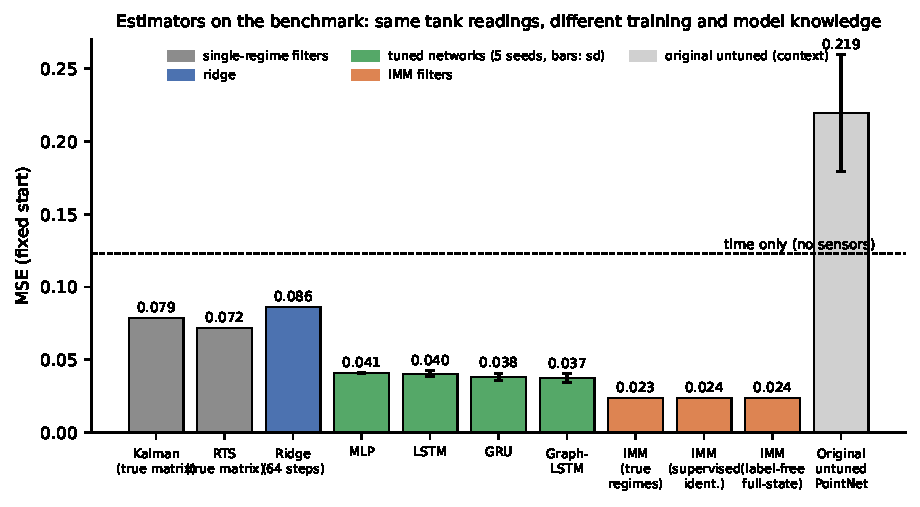
\includegraphics[width=\linewidth]{fig_baselines.pdf}
\caption{Estimators on the fixed-start benchmark, all using the tank readings and masks: single-regime filters, ridge regression, tuned networks (five seeds, error bars show the standard deviation over seeds), IMM filters and for context the best original untuned network. The dashed line is the no-sensor estimator.}
\label{fig:baselines}
\end{figure}

\begin{thebibliography}{9}
\bibitem{kalman1960} R. E. Kalman, ``A New Approach to Linear Filtering and Prediction Problems,'' \emph{Journal of Basic Engineering}, 1960.
\bibitem{rts1965} H. E. Rauch, F. Tung, C. T. Striebel, ``Maximum Likelihood Estimates of Linear Dynamic Systems,'' \emph{AIAA Journal}, 1965.
\bibitem{hermann1977} R. Hermann, A. J. Krener, ``Nonlinear Controllability and Observability,'' \emph{IEEE Transactions on Automatic Control}, 1977.
\bibitem{vanoverschee1996} P. Van Overschee, B. De Moor, \emph{Subspace Identification for Linear Systems}. Springer, 1996.
\bibitem{ljung1999} L. Ljung, \emph{System Identification: Theory for the User}, 2nd ed. Prentice Hall, 1999.
\bibitem{pointnet} C. R. Qi, H. Su, K. Mo, L. J. Guibas, ``PointNet: Deep Learning on Point Sets for 3D Classification and Segmentation,'' in \emph{CVPR}, 2017.
\bibitem{pointnetpp} C. R. Qi, L. Yi, H. Su, L. J. Guibas, ``PointNet++: Deep Hierarchical Feature Learning on Point Sets in a Metric Space,'' in \emph{NeurIPS}, 2017.
\bibitem{kipf2017} T. N. Kipf, M. Welling, ``Semi-Supervised Classification with Graph Convolutional Networks,'' in \emph{ICLR}, 2017.
\bibitem{lakshminarayanan2017} B. Lakshminarayanan, A. Pritzel, C. Blundell, ``Simple and Scalable Predictive Uncertainty Estimation using Deep Ensembles,'' in \emph{NeurIPS}, 2017.
\bibitem{guo2017} C. Guo, G. Pleiss, Y. Sun, K. Q. Weinberger, ``On Calibration of Modern Neural Networks,'' in \emph{ICML}, 2017.
\bibitem{gneiting2007} T. Gneiting, A. E. Raftery, ``Strictly Proper Scoring Rules, Prediction and Estimation,'' \emph{Journal of the American Statistical Association}, 2007.
\bibitem{huber1964} P. J. Huber, ``Robust Estimation of a Location Parameter,'' \emph{Annals of Mathematical Statistics}, 1964.
\bibitem{leth2017farkas} T. Leth, C. Sloth, R. Wisniewski, S. Sankaranarayanan, ``Lyapunov function synthesis --- infeasibility and Farkas' lemma,'' \emph{IFAC-PapersOnLine}, vol. 50, no. 1, pp. 1667--1672, 2017.
\bibitem{misra2020satellite} R. Misra, R. Wisniewski, Ö. Karabacak, ``Sum-of-squares based computation of a Lyapunov function for proving stability of a satellite with electromagnetic actuation,'' \emph{IFAC-PapersOnLine}, vol. 53, no. 2, pp. 7380--7385, 2020.
\bibitem{berry2005} J. W. Berry, L. Fleischer, W. E. Hart, C. A. Phillips, J.-P. Watson, ``Sensor placement in municipal water networks,'' \emph{Journal of Water Resources Planning and Management}, vol. 131, no. 3, pp. 237--243, 2005.
\bibitem{krause2008} A. Krause, J. Leskovec, C. Guestrin, J. VanBriesen, C. Faloutsos, ``Efficient sensor placement optimization for securing large water distribution networks,'' \emph{Journal of Water Resources Planning and Management}, vol. 134, no. 6, pp. 516--526, 2008.
\bibitem{bargiela1989} A. Bargiela, G. D. Hainsworth, ``Pressure and flow uncertainty in water systems,'' \emph{Journal of Water Resources Planning and Management}, vol. 115, no. 2, pp. 212--229, 1989.
\bibitem{preis2011} A. Preis, A. J. Whittle, A. Ostfeld, L. Perelman, ``Efficient hydraulic state estimation technique using reduced models of urban water networks,'' \emph{Journal of Water Resources Planning and Management}, vol. 137, no. 4, pp. 343--351, 2011.
\bibitem{vrachimis2022} S. G. Vrachimis \emph{et al.}, ``Battle of the Leakage Detection and Isolation Methods,'' \emph{Journal of Water Resources Planning and Management}, vol. 148, no. 12, art. 04022068, 2022.
\bibitem{krener2009} A. J. Krener, K. Ide, ``Measures of unobservability,'' in \emph{Proc. 48th IEEE Conference on Decision and Control}, 2009, pp. 6401--6406.
\bibitem{horn2013} R. A. Horn and C. R. Johnson, \emph{Matrix Analysis}, 2nd ed. Cambridge: Cambridge University Press, 2013.
\bibitem{moore1981} B. C. Moore, ``Principal component analysis in linear systems: Controllability, observability, and model reduction,'' \emph{IEEE Transactions on Automatic Control}, vol. 26, no. 1, pp. 17--32, 1981.
\bibitem{stewart1990} G. W. Stewart and J.-G. Sun, \emph{Matrix Perturbation Theory}. Boston: Academic Press, 1990.
\bibitem{rahmani2009} A. Rahmani, M. Ji, M. Mesbahi, M. Egerstedt, ``Controllability of multi-agent systems from a graph-theoretic perspective,'' \emph{SIAM Journal on Control and Optimization}, vol. 48, no. 1, pp. 162--186, 2009.
\bibitem{blom1988} H. A. P. Blom, Y. Bar-Shalom, ``The interacting multiple model algorithm for systems with Markovian switching coefficients,'' \emph{IEEE Transactions on Automatic Control}, vol. 33, no. 8, pp. 780--783, 1988.
\bibitem{barshalom2001} Y. Bar-Shalom, X. R. Li, T. Kirubarajan, \emph{Estimation with Applications to Tracking and Navigation}. Wiley, 2001.
\bibitem{ghahramani2000} Z. Ghahramani, G. E. Hinton, ``Variational learning for switching state-space models,'' \emph{Neural Computation}, vol. 12, no. 4, pp. 831--864, 2000.
\bibitem{fox2011} E. B. Fox, E. B. Sudderth, M. I. Jordan, A. S. Willsky, ``Bayesian nonparametric inference of switching dynamic linear models,'' \emph{IEEE Transactions on Signal Processing}, vol. 59, no. 4, pp. 1569--1585, 2011.
\bibitem{klise2017} K. A. Klise, R. Murray, T. Haxton, ``An overview of the Water Network Tool for Resilience (WNTR),'' in \emph{Proc. World Environmental and Water Resources Congress}, 2017.
\end{thebibliography}

\end{document}
